
%%
%% forked from https://gits-15.sys.kth.se/giampi/kthlatex kthlatex-0.2rc4 on 2020-02-13
%% expanded upon by Gerald Q. Maguire Jr.
%% This template has been adapted by Anders Sjögren to the University
%% Engineering Program in Computer Science at KTH ICT. This adaptation was
%% translation of English headings into Swedish with the addition of Swedish.
%% Many thanks to others who have provided constructive input regarding the template.

% Make it possible to conditionally depend on the TeX engine used
\RequirePackage{ifxetex}
\RequirePackage{ifluatex}
\newif\ifxeorlua
\ifxetex\xeorluatrue\fi
\ifluatex\xeorluatrue\fi

\ifxeorlua
% The following is to ensure that the PDF uses a recent version rather than the typical PDF 1-5
%  This same version of PDF should be set as an option for hyperef

\RequirePackage{expl3}
\RequirePackage{etoolbox}


\ExplSyntaxOn
%pdf_version_gset:n{2.0}
%\pdf_version_gset:n{1.5}

%% Alternatively, if you have a LaTeX newer than June 2022, you can use the following. However, then you have to remove the pdfversion from hyperef. It also breaks hyperxmp. So perhaps it is too early to try using it!
%\DocumentMetadata
%{
%% testphase = phase-I, % tagging without paragraph tagging
% testphase = phase-II % tagging with paragraph tagging and other new stuff.
%pdfversion = 2.0 % pdfversion must be set here.
%}

% Optionally, you can set the uncompress flag to make it easier to examine the PDF
%\pdf_uncompress: % to check the pdf
\ExplSyntaxOff
\else
\RequirePackage{expl3}
\ExplSyntaxOn
%\pdf_version_gset:n{2.0}
\pdf_version_gset:n{1.5}
\ExplSyntaxOff
\fi

%% Define a pair of commands to disable and reenable specific packages - see https://tex.stackexchange.com/questions/39415/unload-a-latex-package
\makeatletter
\newcommand{\disablepackage}[2]{%
  \disable@package@load{#1}{#2}%
}
\newcommand{\reenablepackage}[1]{%
  \reenable@package@load{#1}%
}
\makeatother
%% To avoid the warning: "Package transparent Warning: Loading aborted, because pdfTeX is not running in PDF mode."
\ifxeorlua
\disablepackage{transparent}{}
\fi

%% The template is designed to handle a thesis in English or Swedish
\documentclass[english, bibtex]{kththesis}               % the bibliographic processor to use: biblatex or bibtex
%nomenclature,           % add the option nomenclature
%digitaloutput,          % optimize for digital output (this changes the color palette)
%includeExtraAbstracts, % uncomment to allow abstracts in languages beyond English & Swedish


% if pdflatex \usepackage[utf8]{inputenc}

%% Conventions for todo notes:
% Informational
%% \generalExpl{Comments/directions/... in English}
\newcommand*{\generalExpl}[1]{\todo[inline]{#1}}                

% Language-specific information (currently in English or Swedish)
\newcommand*{\engExpl}[1]{\todo[inline, backgroundcolor=kth-lightgreen40]{#1}} %% \engExpl{English descriptions about formatting}
\newcommand*{\sweExpl}[1]{\todo[inline, backgroundcolor=kth-lightblue40]{#1}}  %% % \sweExpl{Text på svenska}

% warnings
\newcommand*{\warningExpl}[1]{\todo[inline, backgroundcolor=kth-lightred40]{#1}} %% \warningExpl{warnings}

% Uncomment to hide specific comments, to hide **all** ToDos add `final` to
% document class
% \renewcommand\warningExpl[1]{}
% \renewcommand\generalExpl[1]{}
% \renewcommand\engExpl[1]{}
% For example uncommenting the following line hides the Swedish language explanations
% \renewcommand\sweExpl[1]{}


% \usepackage[style=numeric,sorting=none,backend=biber]{biblatex}
\iftoggle{biblatex}{
    %\usepackage[language=english,bibstyle=authoryear,citestyle=authoryear, maxbibnames=99]{biblatex}
    % Alternatively you might use another style, such as IEEE and use citestyle=numeric-comp  to put multiple citations in a single pair of square brackets
    \usepackage[style=ieee,citestyle=numeric-comp]{biblatex}
    \addbibresource{references.bib}
    %\DeclareLanguageMapping{norsk}{norwegian}
}{
    % The line(s) below are for BibTeX
    \bibliographystyle{bibstyle/myIEEEtran}
    %\bibliographystyle{apalike}
}


% include a variety of packages that are useful
\input{lib/includes}
\input{lib/kthcolors}

%\glsdisablehyper
%\makeglossaries
%\makenoidxglossaries
%%%% Local Variables:
%%% mode: latex
%%% TeX-master: t
%%% End:
% The following command is used with glossaries-extra
\setabbreviationstyle[acronym]{long-short}
% The form of the entries in this file is \newacronym{label}{acronym}{phrase}
%                                      or \newacronym[options]{label}{acronym}{phrase}

\newacronym{auprc}{AUPRC}{area under the precision-recall curve}
\newacronym{auroc}{AUROC}{area under the receiver operating characteristic curve}
\newacronym{cpu}{CPU}{central processing unit}
\newacronym{json}{JSON}{JavaScript Object Notation}
\newacronym{API}{API}{application programming interface}
\newacronym{bert}{BERT}{Bidirectional Encoder Representations from Transformers}
\newacronym{gpu}{GPU}{graphics processing unit}
\newacronym[longplural={large language models}]{llm}{LLM}{large language model}
\newacronym{llmjudge}{LLM-as-a-Judge}{large language model as a judge}
\newacronym{qa}{QA}{question answering}
\newacronym{rag}{RAG}{Retrieval-Augmented Generation}
\newacronym{tfidf}{TF-IDF}{term frequency-inverse document frequency}
\newacronym{UN}{UN}{United Nations}
\newacronym{SDG}{SDG}{Sustainable Development Goal}
                %load the acronyms file

\input{lib/defines}  % load some additional definitions to make writing more consistent

% The following is needed in conjunction with generating the DiVA data with abstracts and keywords using the scontents package and a modified listings environment
%\usepackage{listings}   %  already included

\makeatletter
\let\verbatimsc\@undefined
\let\endverbatimsc\@undefined
\lst@AddToHook{Init}{\hyphenpenalty=50\relax}
\makeatother


\lstnewenvironment{verbatimsc}
    {
    \lstset{%
        basicstyle=\ttfamily\tiny,
        backgroundcolor=\color{white},
        %basicstyle=\tiny,
        %columns=fullflexible,
        columns=[l]fixed,
        language=[LaTeX]TeX,
        %numbers=left,
        %numberstyle=\tiny\color{gray},
        keywordstyle=\color{red},
        breaklines=true,                 % sets automatic line breaking
        breakatwhitespace=true,          % sets if automatic breaks should only happen at whitespace
        %keepspaces=false,
        breakindent=0em,
        %fancyvrb=true,
        frame=none,                     % turn off any box
        postbreak={}                    % turn off any hook arrow for continuation lines
    }
}{}

%% Add some more keywords to bring out the structure more
\lstdefinestyle{[LaTeX]TeX}{
morekeywords={begin, todo, textbf, textit, texttt}
}

%% definition of new command for bytefield package
\newcommand{\colorbitbox}[3]{%
	\rlap{\bitbox{#2}{\color{#1}\rule{\width}{\height}}}%
	\bitbox{#2}{#3}}




% define a left aligned table cell that is ragged right
\newcolumntype{L}[1]{>{\raggedright\let\newline\\\arraybackslash\hspace{0pt}}p{#1}}

% Because backref is not compatible with biblatex
\iftoggle{biblatex}{
    \usepackage[plainpages=false]{hyperref}
}{
    \usepackage[
    backref=page,
    pagebackref=false,
    plainpages=false,
                            % PDF related options
    unicode=true,           % Unicode encoded PDF strings
    bookmarks=true,         % generate bookmarks in PDF files
    bookmarksopen=false,    % Do not automatically open the bookmarks in the PDF reading program
    pdfpagemode=UseNone,    % None, UseOutlines, UseThumbs, or FullScreen
    destlabel,              % better naming of destinations
    pdfencoding=auto,       % for unicode in 
    ]{hyperref}
   %% Removed use of backref package as it is incompatible with using attachfile
}

\usepackage[all]{hypcap}	%% prevents an issue related to hyperref and caption linking

%% Acronyms
% note that nonumberlist - removes the cross references to the pages where the acronym appears
% note that super will set the descriptions text aligned
% note that nomain - does not produce a main glossary, thus only acronyms will be in the glossary
% note that nopostdot - will prevent there being a period at the end of each entry
\usepackage[acronym, style=super, section=section, nonumberlist, nomain,
nopostdot]{glossaries}
\setlength{\glsdescwidth}{0.75\textwidth}
\usepackage[]{glossaries-extra}
\ifinswedish
    %\usepackage{glossaries-swedish}
\fi

%% For use with the README_notes
% Define a new type of glossary so that the acronyms defined in the README_notes document can be distinct from those in the thesis template
% the tlg, tld, and dn will be the file extensions used for this glossary
\newglossary[tlg]{readme}{tld}{tdn}{README acronyms}


\input{lib/includes-after-hyperref}

%\glsdisablehyper
\makeglossaries
%\makenoidxglossaries

% The following bit of ugliness is because of the problems PDFLaTeX has handling a non-breaking hyphen
% unless it is converted to UTF-8 encoding.
% If you do not use such characters in your acronyms, this could be simplified to just include the acronyms file.
\ifxeorlua
%%% Local Variables:
%%% mode: latex
%%% TeX-master: t
%%% End:
% The following command is used with glossaries-extra
\setabbreviationstyle[acronym]{long-short}
% The form of the entries in this file is \newacronym{label}{acronym}{phrase}
%                                      or \newacronym[options]{label}{acronym}{phrase}

\newacronym{auprc}{AUPRC}{area under the precision-recall curve}
\newacronym{auroc}{AUROC}{area under the receiver operating characteristic curve}
\newacronym{cpu}{CPU}{central processing unit}
\newacronym{json}{JSON}{JavaScript Object Notation}
\newacronym{API}{API}{application programming interface}
\newacronym{bert}{BERT}{Bidirectional Encoder Representations from Transformers}
\newacronym{gpu}{GPU}{graphics processing unit}
\newacronym[longplural={large language models}]{llm}{LLM}{large language model}
\newacronym{llmjudge}{LLM-as-a-Judge}{large language model as a judge}
\newacronym{qa}{QA}{question answering}
\newacronym{rag}{RAG}{Retrieval-Augmented Generation}
\newacronym{tfidf}{TF-IDF}{term frequency-inverse document frequency}
\newacronym{UN}{UN}{United Nations}
\newacronym{SDG}{SDG}{Sustainable Development Goal}
                %load the acronyms file
\else
\input{lib/acronyms-for-pdflatex}
\fi

% place holders for languages lacking .lbx files
\input{lib/placeHolder_lbx_files}

% insert the configuration information with author(s), examiner, supervisor(s), ...
\input{custom_configuration}

% read in the plain text definitions, if they exist
\IfFileExists{custom_configuration_plaintext.tex}{\input{custom_configuration_plaintext.tex}}{}


% Enter the English and Swedish keywords here for use in the PDF metadata _and_ for later use
% following the respective abstract.
% Try to put the words in the same order in both languages to facilitate matching. For example:
\EnglishKeywords{Retrieval-Augmented Generation, Graph RAG, Query routing, LightRAG, 2WikiMultihopQA, LLM-as-a-Judge}
\SwedishKeywords{Retrieval-Augmented Generation, grafbaserad RAG, frågeroutning, LightRAG, 2WikiMultihopQA, LLM-som-domare}

%%%%% For the oral presentation
%% Add this information once your examiner has scheduled your oral presentation
\presentationDateAndTimeISO{}
\presentationLanguage{}  % generally: eng or swe
\presentationRoom{}
\presentationAddress{}
\presentationCity{Stockholm}

% When there are multiple opponents, separate their names with '\&'
% Opponent's information
%\opponentsNames{A. B. Normal \& A. X. E. Normalè}
\opponentsNames{}

% It is possible to have a cover illustration
%\coverIllustration{figures/image1.png}
% if so, the author might acknowledge this or give the copyright information for it with:
%\coverIllustrationCredit{A. B. Normal}

% Once a thesis is approved by the examiner, add the TRITA number
% The TRITA number for a thesis consists of two parts: a series (unique to each school)
% and the number in the series, which is formatted as the year followed by a colon and
% then a unique series number for the thesis - starting with 1 each year.
%\trita{TRITA -- XXX-EX}{2026:0000}

% Put the title, author, and keyword information into the PDF meta information
\input{lib/pdf_related_includes}


% the custom colors and the commands are defined in defines.tex    
\hypersetup{
	colorlinks  = true,
	breaklinks  = true,
	linkcolor   = \linkscolor,
	urlcolor    = \urlscolor,
	citecolor   = \refscolor,
	anchorcolor = black
}

\ifnomenclature
% The following lines make the page numbers and equations hyperlinks in the Nomenclature list
\renewcommand*{\pagedeclaration}[1]{\unskip, \dotfill\hyperlink{page.#1}{page\nobreakspace#1}}
% The following does not work correctly, as the name of the cross-reference is incorrect
%\renewcommand*{\eqdeclaration}[1]{, see equation\nobreakspace(\hyperlink{equation.#1}{#1})}

% You can also change the page heading for the nomenclature
\renewcommand{\nomname}{List of Symbols Used}

% You can even add customization text before the list
\renewcommand{\nompreamble}{The following symbols will be later used within the body of the thesis.}
\makenomenclature
\fi

%
% The commands below are to configure JSON listings
% 
% format for JSON listings
\colorlet{punct}{red!60!black}
\definecolor{delim}{RGB}{20,105,176}
\definecolor{numb}{RGB}{106, 109, 32}
\definecolor{string}{RGB}{0, 0, 0}

\lstdefinelanguage{json}{
    numbers=none,
    numberstyle=\small,
    frame=none,
    rulecolor=\color{black},
    showspaces=false,
    showtabs=false,
    breaklines=true,
    postbreak=\raisebox{0ex}[0ex][0ex]{\ensuremath{\color{gray}\hookrightarrow\space}},
    breakatwhitespace=true,
    basicstyle=\ttfamily\small,
    extendedchars=false,
    upquote=true,
    morestring=[b]",
    stringstyle=\color{string},
    literate=
     *{0}{{{\color{numb}0}}}{1}
      {1}{{{\color{numb}1}}}{1}
      {2}{{{\color{numb}2}}}{1}
      {3}{{{\color{numb}3}}}{1}
      {4}{{{\color{numb}4}}}{1}
      {5}{{{\color{numb}5}}}{1}
      {6}{{{\color{numb}6}}}{1}
      {7}{{{\color{numb}7}}}{1}
      {8}{{{\color{numb}8}}}{1}
      {9}{{{\color{numb}9}}}{1}
      {:}{{{\color{punct}{:}}}}{1}
      {,}{{{\color{punct}{,}}}}{1}
      {\{}{{{\color{delim}{\{}}}}{1}
      {\}}{{{\color{delim}{\}}}}}{1}
      {[}{{{\color{delim}{[}}}}{1}
      {]}{{{\color{delim}{]}}}}{1}
      {’}{{\char13}}1,
}

\lstdefinelanguage{XML}
{
  basicstyle=\ttfamily\color{blue}\bfseries\small,
  morestring=[b]",
  morestring=[s]{>}{<},
  morecomment=[s]{<?}{?>},
  stringstyle=\color{black},
  identifierstyle=\color{blue},
  keywordstyle=\color{cyan},
  breaklines=true,
  postbreak=\raisebox{0ex}[0ex][0ex]{\ensuremath{\color{gray}\hookrightarrow\space}},
  breakatwhitespace=true,
  morekeywords={xmlns,version,type}% list your attributes here
}

% If you use both listing and lstlisting environments - the following makes them both use the same counter and the same formatting in the List of Listings
\makeatletter
\AtBeginDocument{\let\c@listing\c@lstlisting}
\AtBeginDocument{\let\l@listing\l@lstlisting}
\makeatother

% Change the heading for the "List of Listings" to simply "Listings"
\renewcommand{\lstlistlistingname}{Listings}

% number each listing within the chapter
\numberwithin{listing}{chapter}

\usepackage{subfiles}

% To have Creative Commons (CC) license and logos use the doclicense package
% Note that the lowercase version of the license has to be used in the modifier
% i.e., one of by, by-nc, by-nd, by-nc-nd, by-sa, by-nc-sa, zero.
% For background see:
% https://www.kb.se/samverkan-och-utveckling/oppen-tillgang-och-bibsamkonsortiet/open-access-and-bibsam-consortium/open-access/creative-commons-faq-for-researchers.html
% https://kib.ki.se/en/publish-analyse/publish-your-article-open-access/open-licence-your-publication-cc
\begin{comment}
\usepackage[
    type={CC},
    %modifier={by-nc-nd},
    %version={4.0},
    modifier={by-nc},
    imagemodifier={-eu-88x31},  % to get Euro symbol rather than Dollar sign
    hyphenation={RaggedRight},
    version={4.0},
    %modifier={zero},
    %version={1.0},
]{doclicense}
\end{comment}
\listfiles

\begin{document}
%\selectlanguage{swedish}
%
\selectlanguage{english}

%%% Set the numbering for the title page to a numbering series not in the preface or body
\pagenumbering{alph}
\kthcover
\clearpage\thispagestyle{empty}\mbox{} % empty back of front cover
\titlepage

% If you do not want to have a bookinfo page, comment out the line saying \bookinfopage and add a \cleardoublepage
% If you want a bookinfo page: you will get a copyright notice, unless you have used the doclicense package in which case you will get a Creative Commons license. To include the doclicense package, uncomment the configuration of this package above and configure it with your choice of license.
\bookinfopage

% Frontmatter includes the abstracts and table-of-contents
\frontmatter
\setcounter{page}{1}
\begin{abstract}
% The first abstract should be in the language of the thesis.
% Abstract fungerar på svenska också.
  \markboth{\abstractname}{}
\begin{scontents}[store-env=lang]
eng
\end{scontents}
%%% The contents of the abstract (between the begin and end of scontents) will be saved in LaTeX format
%%% and output on the page(s) at the end of the thesis with information for DiVA facilitating the correct
%%% entry of the meta data for your thesis.
%%% These page(s) will be removed before the thesis is inserted into DiVA.
\engExpl{All theses at KTH are \textbf{required} to have an abstract in both \textit{English} and \textit{Swedish}.}

\engExpl{Exchange students may want to include one or more abstracts in the language(s) used in their home institutions to avoid the need to write another thesis when returning to their home institution.}

\generalExpl{Keep in mind that most of your potential readers are only going to read your \texttt{title} and \texttt{abstract}. This is why the abstract must give them enough information so that they can decide if this document is relevant to them or not. Otherwise, the likely default choice is to ignore the rest of your document.\\
An abstract should stand on its own, \ie no citations, cross-references to the body of the document, acronyms must be spelled out, \ldots .\\Write this early and revise as necessary. This will help keep you focused on what you are trying to do.}

\begin{scontents}[store-env=abstracts,print-env=true]
\generalExpl{Enter your abstract here!}
An abstract is (typically) about 250 and 350 words (1/2 A4-page) with the following components:
% key parts of the abstract
\begin{itemize}
  \item What is the topic area? (optional) Introduces the subject area for the project.
  \item Short problem statement
  \item Why was this problem worth a Bachelor's/Master’s thesis project? (\ie, why is the problem both significant and of a suitable degree of difficulty for a Bachelor's/Master’s thesis project? Why has no one else solved it yet?)
  \item How did you solve the problem? What was your method/insight?
  \item Results/Conclusions/Consequences/Impact: What are your key results/\linebreak[4]conclusions? What will others do based on your results? What can be done now that you have finished - that could not be done before your thesis project was completed?
\end{itemize}

\end{scontents}
\engExpl{The following are some notes about what can be included (in terms of LaTeX) in your abstract.}
Choice of typeface with \textbackslash textit, \textbackslash textbf, and \textbackslash texttt:  \textit{x}, \textbf{x}, and \texttt{x}.

Text superscripts and subscripts with \textbackslash textsubscript and \textbackslash textsuperscript: A\textsubscript{x} and A\textsuperscript{x}.

Some symbols that you might find useful are available, such as: \textbackslash textregistered, \textbackslash texttrademark, and \textbackslash textcopyright. For example, 
the copyright symbol: \textbackslash textcopyright Maguire 2022 results in \textcopyright Maguire 2022. Additionally, here are some examples of text superscripts (which can be combined with some symbols): \textbackslash textsuperscript\{99m\}Tc, A\textbackslash textsuperscript\{*\}, A\textbackslash textsuperscript\{\textbackslash textregistered\}, and A\textbackslash texttrademark resulting in \textsuperscript{99m}Tc, A\textsuperscript{*}, A\textsuperscript{\textregistered}, and A\texttrademark. Two examples of subscripts are: H\textbackslash textsubscript\{2\}O and CO\textbackslash textsubscript\{2\} which produce  H\textsubscript{2}O and CO\textsubscript{2}.

You can use simple environments with begin and end: itemize and enumerate and within these use instances of \textbackslash item.

The following commands can be used: \textbackslash eg, \textbackslash Eg, \textbackslash ie, \textbackslash Ie, \textbackslash etc, and \textbackslash etal: \eg, \Eg, \ie, \Ie, \etc, and \etal.

The following commands for numbering with lowercase Roman numerals: \textbackslash first, \textbackslash Second, \textbackslash third, \textbackslash fourth, \textbackslash fifth, \textbackslash sixth, \textbackslash seventh, and \textbackslash eighth: \first, \Second, \third, \fourth, \fifth, \sixth, \seventh, and \eighth. Note that the second case is set with a capital 'S' to avoid conflicts with the use of second as a unit in the \texttt{siunitx} package.

Equations using \textbackslash( xxxx \textbackslash) or \textbackslash[ xxxx \textbackslash] can be used in the abstract. For example: \( (C_5O_2H_8)_n \)
or \[ \int_{a}^{b} x^2 \,dx \]
Note that you \textbf{cannot} use an equation between dollar signs.


Even LaTeX comments can be handled by using a backslash to quote the percent symbol, for example: \% comment.
Note that one can include percentages, such as: 51\% or \SI{51}{\percent}.

\subsection*{Keywords}
\begin{scontents}[store-env=keywords,print-env=true]
% If you set the EnglishKeywords earlier, you can retrieve them with:
\InsertKeywords{english}
% If you did not set the EnglishKeywords earlier then simply enter the keywords here:
% comma separate keywords, such as: Canvas Learning Management System, Docker containers, Performance tuning
\end{scontents}
\engExpl{\textbf{Choosing good keywords can help others to locate your paper, thesis, dissertation, \ldots and related work.}}
Choose the most specific keyword from those used in your domain, see for example: the ACM Computing Classification System ({\small \url{https://www.acm.org/publications/computing-classification-system/how-to-use})},
the IEEE Taxonomy ({\small \url{https://www.ieee.org/publications/services/thesaurus-thank-you.html}}), PhySH (Physics Subject Headings)\linebreak[4] ({\small \url{https://physh.aps.org/}}), \ldots or keyword selection tools such as the  National Library of Medicine's Medical Subject Headings (MeSH)  ({\small \url{https://www.nlm.nih.gov/mesh/authors.html}}) or Google's Keyword Tool ({\small \url{https://keywordtool.io/}})\\

\textbf{Formatting the keywords}:
\begin{itemize}
  \item The first letter of a keyword should be set with a capital letter and proper names should be capitalized as usual.
  \item Spell out acronyms and abbreviations.
  \item Avoid "stop words" - as they generally carry little or no information.
  \item List your keywords separated by commas (``,'').
\end{itemize}    
Since you should have both English and Swedish keywords - you might think of ordering the keywords in corresponding order (\ie, so that the n\textsuperscript{th} word in each list correspond) - this makes it easier to mechanically find matching keywords.
\end{abstract}
\cleardoublepage
\babelpolyLangStart{swedish}
\begin{abstract}
    \markboth{\abstractname}{}
\begin{scontents}[store-env=lang]
swe
\end{scontents}
\warningExpl{Inside the following scontents environment, you cannot use a \textbackslash include{filename} as the command rather than the file contents will end up in the for DiVA information. Additionally, you should not use a straight double quote character in the abstracts or keywords, use two single quote characters instead.}
\sweExpl{Alla avhandlingar vid KTH \textbf{måste ha} ett abstrakt på både \textit{engelska} och \textit{svenska}.\\
Om du skriver din avhandling på svenska ska detta göras först (och placera det som det första abstraktet) - och du bör revidera det vid behov.}

\engExpl{If you are writing your thesis in English, you can leave this until the draft version that goes to your opponent for the written opposition. In this way, you can provide the English and Swedish abstract/summary information that can be used in the announcement for your oral presentation.\\If you are writing your thesis in English, then this section can be a summary targeted at a more general reader. However, if you are writing your thesis in Swedish, then the reverse is true – your abstract should be for your target audience, while an English summary can be written targeted at a more general audience.\\This means that the English abstract and Swedish sammnfattning  
or Swedish abstract and English summary need not be literal translations of each other.}

\warningExpl{Do not use the \textbackslash glspl\{\} command in an abstract that is not in English, as my programs do not know how to generate plurals in other languages. Instead, you will need to spell these terms out or give the proper plural form. In fact, it is a good idea not to use the glossary commands at all in an abstract/summary in a language other than the language used in the \texttt{acronyms.tex file} - since the glossary package does \textbf{not} support use of more than one language.}

\engExpl{The abstract in the language used for the thesis should be the first abstract, while the Summary/Sammanfattning in the other language can follow}
\begin{scontents}[store-env=abstracts,print-env=true]
\generalExpl{Enter your Swedish abstract or summary here!}

\end{scontents}
\subsection*{Nyckelord}
\begin{scontents}[store-env=keywords,print-env=true]
% SwedishKeywords were set earlier, hence we can use alternative 2
\InsertKeywords{swedish}
\end{scontents}
\sweExpl{Nyckelord som beskriver innehållet i uppsatsen eller rapporten}
\end{abstract}
\cleardoublepage
\babelpolyLangStop{swedish}
% Note that the \cleardoublepage has to be before the 
% \babelpolyLangStop - otherwise the running headers will not be in the correct language


\engExpl{If you add the class option \texttt{includeExtraAbstracts} in your \texttt{docuemntclass}, then you can enable abstracts/summaries in a number of languages. Include those versions of abstracts that you need.}
\generalExpl{If you are an exchange student, use the relevant language or languages for abstracts for your home university, as this will often avoid the need for writing another thesis for your home university.}
\generalExpl{If you are fluent in other languages, feel free to add the abstracts in one or more of them.}

\engExpl{The set of languages that can be easily included are based on those languages that were used in theses at KTH in the period 2018-2019, along with several others that have been used in theses since.}
\warningExpl{Note that you may need to augment the set of languages used in \texttt{polyglossia} or
\texttt{babel} (see the file \texttt{kththesis.cls}). If you add a new language, when specifying the language for the abstract, use the three-letter ISO 639-2 Code – specifically the "B" (bibliographic) variant of these codes (note that this is the same language code used in DiVA).}

\cleardoublepage
\iftoggle{includeExtraAbstracts}{
% To include abstracts in languages other than English and Swedish:
%  1. Ensure 'includeExtraAbstracts' is an active option in \documentclass.
%  2. Uncomment the relevant '\input' line(s) below.
%  3. Edit the content within the corresponding file in the 'Additional_Abstracts/' folder.
% Include only the abstracts that you want and fill them in as appropriate
% The template will automatically include the information that you entered
%
% Languages in frequency order based on DiVA data from 2025-05-28

% --- Include Spanish abstract ---
%\input{Additional_Abstracts/abstract_spanish}

% --- Include French abstract ---
%\input{Additional_Abstracts/abstract_french}

% --- Include German abstract ---
%\input{Additional_Abstracts/abstract_german}

% --- Include Italian abstract ---
%\input{Additional_Abstracts/abstract_italian}

% --- Include Chinese abstract ---
%\input{Additional_Abstracts/abstract_chinese}

% --- Include Norwegian abstract ---
%\input{Additional_Abstracts/abstract_norweign}

% --- Include Catalan abstract ---
%\input{Additional_Abstracts/abstract_catalan}

% --- Include Finnish abstract ---
%\input{Additional_Abstracts/abstract_finnish}

% --- Include Portuguese abstract ---
%\input{Additional_Abstracts/abstract_chinese}

% --- Include Dutch abstract ---
%\input{Additional_Abstracts/abstract_dutch}

% --- Include Swahili / Kiswahili summary ---
%\input{Additional_Abstracts/abstract_swahili}

% --- Include Russian summary ---
%\input{Additional_Abstracts/abstract_russian}

% --- Include Polish abstract ---
%\input{Additional_Abstracts/abstract_polishn}

% --- Include Ukrainian abstract ---
%\input{Additional_Abstracts/abstract_ukrainian}

% --- Include Hindi abstract ---
%\input{Additional_Abstracts/abstract_hindi}

% --- Include Danish abstract ---
%\input{Additional_Abstracts/abstract_danish}

% --- Include Estonian abstract ---
%\input{Additional_Abstracts/abstract_estonian}

% --- Include Slovak abstract ---
%\input{Additional_Abstracts/abstract_slovak}

% --- Include Serbian abstract ---
%\input{Additional_Abstracts/abstract_serbian}

% --- Include Bosnian abstract ---
%\input{Additional_Abstracts/abstract_bosnian}

%% missing many languages



}{} %% End the iiftoggle{includeExtraAbstracts}

\section*{Acknowledgments}
\markboth{Acknowledgments}{}
\sweExpl{Författarnas tack}

\engExpl{It is nice to acknowledge the people that have helped you. It is
  also necessary to acknowledge any special permissions that you have gotten –
  for example, getting permission from the copyright owner to reproduce a
  figure. In this case, you should acknowledge them and this permission here
  and in the figure’s caption. \\
  Note: If you do \textbf{not} have the copyright owner’s permission, then you \textbf{cannot} use any copyrighted figures/tables/\ldots . Unless stated otherwise all figures/tables/\ldots are generally copyrighted.
}
\sweExpl{I detta kapitel kan du ev nämna något om
  din bakgrund om det påverkar rapporten på något sätt. Har du t ex inte
  möjlighet att skriva perfekt svenska för att du är nyanländ till landet kan
  det vara på sin plats att nämna detta här. OBS, detta får dock inte vara en
  ursäkt för att lämna in en rapport med undermåligt språk, undermålig grammatik och
  stavning (t ex får fel som en automatisk stavningskontroll och
  grammatikkontroll kan upptäcka inte förekomma)\\
En dualism som måste hanteras i hela rapporten och projektet
}

\engExpl{To ensure academic transparency, you must report whether and how generative AI has been used in your examinable work.  This includes any new content, including, but not limited text, images, tables, or code.}
\sweExpl{För att säkerställa akademisk transparens måste du rapportera om och hur generativ AI har använts i ditt examinerbara arbete. Detta inkluderar allt nytt innehåll, inklusive, men inte begränsat till, text, bilder, tabeller eller kod.}

I would like to thank xxxx for having yyyy. Or in the case of two authors:\\
We would like to thank xxxx for having yyyy.

\acknowlegmentssignature

\fancypagestyle{plain}{}
\renewcommand{\chaptermark}[1]{ \markboth{#1}{}} 
\tableofcontents
  \markboth{\contentsname}{}

\cleardoublepage
\listoffigures

\cleardoublepage

\listoftables
\cleardoublepage
\lstlistoflistings\engExpl{If you have listings in your thesis. If not, then remove this preface page.}
\cleardoublepage
% Align the text expansion of the glossary entries
\newglossarystyle{mylong}{%
  \setglossarystyle{long}%
  \renewenvironment{theglossary}%
     {\begin{longtable}[l]{@{}p{\dimexpr 2cm-\tabcolsep}p{0.8\hsize}}}% <-- change the value here
     {\end{longtable}}%
 }
%\glsaddall
%\printglossaries[type=\acronymtype, title={List of acronyms}]
\printglossary[style=mylong, type=\acronymtype, title={List of acronyms and abbreviations}]
%\printglossary[type=\acronymtype, title={List of acronyms and abbreviations}]

%\printnoidxglossary[style=mylong, title={List of acronyms and abbreviations}]
\engExpl{The list of acronyms and abbreviations should be in alphabetical order based on the spelling of the acronym or abbreviation.
}

% if the nomenclature option was specified, then include the nomenclature page(s)
\ifnomenclature
    \cleardoublepage
    % Output the nomenclature list
    \printnomenclature
\fi

%% The following label is essential to know the page number of the last page of the preface
%% It is used to compute the data for the "For DIVA" pages
\label{pg:lastPageofPreface}
% Mainmatter is where the actual contents of the thesis goes
\mainmatter
\glsresetall
\glsunset{API}
\glsunset{auprc}
\glsunset{bert}
\glsunset{gpu}
\glsunset{llm}
\glsunset{llmjudge}
\glsunset{qa}
\glsunset{rag}
\glsunset{tfidf}
\renewcommand{\chaptermark}[1]{\markboth{#1}{}}
\selectlanguage{english}
\chapter{Introduction}
\label{ch:introduction}

This chapter introduces the thesis topic and motivates the problem studied in the project. Section~\ref{sec:background} gives the background to retrieval-augmented question answering and the cost of different retrieval modes. Section~\ref{sec:problem} defines the problem and research question. Section~\ref{sec:purpose} states the purpose of the work, Section~\ref{sec:goals} presents the goals, Section~\ref{sec:researchMethodology} outlines the research methodology, Section~\ref{sec:delimitations} defines the delimitations, and Section~\ref{sec:structure} describes the structure of the rest of the thesis.

\section{Background}
\label{sec:background}

\Gls{rag} systems can answer questions over information that is not contained in a language model's parameters, but the retrieval strategy itself becomes a design choice with practical consequences. This thesis studies that choice as a supervised routing problem. Given only a query, can a lightweight model predict whether cheap vector retrieval is sufficient or whether a more expensive graph-enhanced retrieval mode is required?

\Gls{rag} has become a common architecture for grounding \gls{llm} outputs in external documents, especially when the relevant information is private, domain-specific, or changes after model pretraining \cite{gao2023ragsurvey}. A typical \gls{rag} system retrieves text passages from a corpus and conditions the generator on those passages. This makes the language model less dependent on memorized knowledge and allows it to answer questions over a controlled knowledge base.

The simplest and most common retrieval layer is based on vector similarity search over document chunks. This approach is efficient and often effective for local factual questions, but it can struggle when a query depends on linking evidence across documents, resolving relationships between entities, or comparing distributed attributes. Graph-enhanced \gls{rag} systems address this limitation by introducing structured representations of entities, relations, or higher-level document organization. Recent systems such as GraphRAG and LightRAG show how graph-based structure can support retrieval beyond isolated nearest-neighbor chunks \cite{edge2024graphrag,lightrag2024}.

Richer retrieval is not free. Graph construction, graph traversal, larger context assembly, and additional language-model calls can increase execution time. In industrial settings such as Ericsson, where internal technical repositories are large and fragmented, this cost matters because graph-enhanced retrieval may improve answer quality for difficult questions, but applying it to every query would waste computation on questions that could already be answered by cheaper vector retrieval \cite{jeong2024adaptiverag,hu2024routerbench}.

This motivates adaptive retrieval. Work such as Self-RAG and Adaptive-RAG argues that retrieval behavior should depend on the query rather than follow a fixed policy for all inputs \cite{asai2023selfrag,jeong2024adaptiverag}. More broadly, model and system routing work frames this as a cost--performance decision where different execution paths have different expected benefits and costs, and a router should select the path that is appropriate for the input \cite{hu2024routerbench}.

The specific question studied in this thesis is narrower than general model routing. Instead of routing between different language models, the thesis routes between retrieval modes inside a fixed Hybrid \gls{rag} setting. The low-cost path is LightRAG's \emph{Naive} mode, used here as a vector-retrieval baseline, and the high-cost path is LightRAG's \emph{Mix} mode, which combines vector retrieval with graph-enhanced retrieval. The routing layer is intentionally lightweight. Since the router is meant to reduce retrieval and generation runtime, it should not itself require a large decoder model. Prior work on encoder-only classification supports this design choice for narrow text-classification tasks \cite{benayas2024encoder}.

\section{Problem}
\label{sec:problem}

Hybrid \gls{rag} systems expose a practical tension between retrieval quality and retrieval cost. A cheap vector-based path can be sufficient for many questions, while a graph-enhanced path can be useful when the answer depends on relationships or evidence distributed across several documents. However, a static retrieval policy cannot exploit this distinction. Always using the cheap path risks missing cases where structured retrieval is needed, while always using the expensive path introduces unnecessary latency and computation for easier queries.

This thesis focuses on that decision point. In LightRAG, it is operationalized as a choice between \emph{Naive} retrieval, used as the lower-cost vector path, and \emph{Mix} retrieval, used as the more expensive graph-enhanced path. Existing work motivates both graph-based \gls{rag} and adaptive retrieval \cite{edge2024graphrag,lightrag2024,asai2023selfrag,jeong2024adaptiverag}, but it does not fully answer whether this particular retrieval-mode choice can be predicted before retrieval from the query text alone.

\subsection{Original problem and definition}
\label{sec:researchQuestion}

The practical motivation comes from industrial \gls{qa} over large technical repositories. Ericsson works with internal documentation where relevant information can be fragmented across documents and absent from public language-model pretraining. In such a setting, \gls{rag} is needed for grounding, but graph-enhanced retrieval should ideally be used only when the cheaper vector path is insufficient.

The original engineering problem is therefore to decide, for a given query in a Hybrid \gls{rag} system, whether cheap vector retrieval is sufficient or whether graph-enhanced retrieval is required. The decision must be made before the expensive retrieval path is executed. Since the router is meant to reduce runtime, it should itself remain lightweight. This thesis therefore uses a ModernBERT-based query classifier rather than a large general-purpose \gls{llm} router \cite{benayas2024encoder,warner2024modernbert}.

\subsection{Scientific and engineering issues}
\label{sec:scientificEngineeringIssues}

The scientific issue is the predictability of retrieval need. If the distinction between vector-sufficient and graph-required queries is mainly determined by corpus state after retrieval, then a query-only router should not perform reliably. If the distinction is partly reflected in the query itself, then a supervised classifier may learn a useful decision boundary.

The engineering issue is that the benchmark provides answer supervision but not routing supervision. This thesis therefore constructs routing labels by executing both retrieval modes on 2WikiMultihopQA and comparing the outputs against benchmark answers using \gls{llmjudge}, while treating the judge as a fallible labeling instrument rather than unquestioned ground truth \cite{ho2020twowiki,zheng2023judge}.

\subsubsection{Research question}

Within a fixed Hybrid \gls{rag} setting, how predictable is the distinction between queries for which vector retrieval is sufficient and queries for which graph-enhanced retrieval is required, based on the query text alone?

\section{Purpose}
\label{sec:purpose}
The purpose of this thesis is to investigate whether retrieval-mode selection in a Hybrid \gls{rag} system can be made adaptive without moving the routing decision into another expensive model call. The intended improvement is practical. Graph-enhanced retrieval should be used when it is needed, but avoided when vector retrieval is already sufficient.

For an industrial setting such as Ericsson, this matters because internal technical documentation can be large, fragmented, and absent from public language-model pretraining. High-quality grounded \gls{qa} is useful in such an environment, but indiscriminately applying the most expensive retrieval strategy creates unnecessary latency and runtime cost. A successful router would support more efficient \gls{qa} by reducing redundant use of graph-enhanced retrieval while preserving access to it for queries that require structured evidence.

The academic purpose is to study retrieval-mode selection as a narrow supervised prediction problem. The thesis does not aim to prove that graph retrieval is universally superior, nor that LightRAG is the best possible \gls{rag} framework. Instead, it asks whether the need for graph-enhanced retrieval is predictable enough from the query text that a lightweight classifier can serve as a useful control layer. This makes the contribution empirical because the thesis evaluates whether the distinction between vector-sufficient and graph-required queries can be learned in a fixed experimental setting.



\section{Goals}
\label{sec:goals}
The main goal of the project is to design and evaluate a learned routing layer that predicts whether a query should use LightRAG's \emph{Naive} or \emph{Mix} retrieval mode. The four concrete objectives are listed below.

\begin{enumerate}
\item Implement a reproducible pipeline for preparing 2WikiMultihopQA samples, indexing them in LightRAG, and executing both \emph{Naive} and \emph{Mix} retrieval modes.
\item Construct a supervised routing dataset by labeling each query according to the minimum viable retrieval mode, using \gls{llmjudge} to compare retrieval outputs against benchmark answers.
\item Train lightweight query-only routers, including a ModernBERT-based classifier and a classical \gls{tfidf} logistic-regression baseline, to predict whether graph-enhanced retrieval is required.
\item Evaluate the routers both as held-out classifiers using metrics such as \gls{auprc} and as thresholded routing policies through offline simulation against majority-class, always-\emph{Naive}, and always-\emph{Mix} baselines.
\end{enumerate}

\section{Research Methodology}
\label{sec:researchMethodology}

This thesis will conduct a quantitative empirical study using the public 2WikiMultihopQA benchmark for model training and evaluation. The study will use LightRAG as a fixed Hybrid \gls{rag} system and compare the \emph{Naive} and \emph{Mix} retrieval modes for each query. The generated answers will be evaluated against benchmark answers with an \gls{llmjudge} procedure, producing routing labels that indicate whether vector retrieval was sufficient or graph-enhanced retrieval was required.

The resulting labels will be used to train lightweight query-only routers, including a ModernBERT-based classifier and a \gls{tfidf} logistic-regression baseline. Evaluation will be done on held-out data using classification metrics such as \gls{auprc}, precision, recall, and F1. These metrics estimate how reliably the router predicts the judged routing decision.

To connect the classifier results to system efficiency, the predicted probabilities will also be evaluated as routing policies. Different thresholds will be compared against static baselines that always use \emph{Naive} or always use \emph{Mix}, using measured execution times and judged answer outcomes. These comparisons will be used to answer the research question about whether query-only routing can improve the efficiency--accuracy trade-off in the fixed Hybrid \gls{rag} setting.

\section{Delimitations}
\label{sec:delimitations}

The thesis is deliberately limited to query-only retrieval-mode routing. The router receives the query text as input and does not inspect retrieved documents, intermediate graph state, answer drafts, or model uncertainty after generation. This delimitation makes the routing problem cheaper and cleaner, but it also means the thesis does not evaluate routers that adapt after retrieval has already begun.

The experimental retrieval setting is LightRAG, and the retrieval actions are limited to \emph{Naive} and \emph{Mix}. These modes operationalize the broader distinction between vector retrieval and graph-enhanced retrieval, but the thesis does not claim that results transfer automatically to every Hybrid \gls{rag} framework or every possible retrieval strategy.

The primary benchmark is 2WikiMultihopQA \cite{ho2020twowiki}. This provides public questions, answers, and supporting evidence, which makes the experiment reproducible and avoids making the thesis dependent on confidential data. Ericsson documentation motivates the industrial problem and may support future external validation, but it is not the core benchmark for the thesis contribution.

The routing labels are generated with \gls{llmjudge} and are therefore treated as judged supervision rather than absolute ground truth. The thesis excludes cases where neither retrieval mode is sufficient, and it does not attempt to solve answer generation failures that are independent of the routing decision.

\section{Structure of the thesis}
\label{sec:structure}

Chapter~\ref{ch:background} presents the technical and scientific background on \gls{rag}, graph-enhanced retrieval, adaptive retrieval, query routing, ModernBERT, and related work. Chapter~\ref{ch:methods} describes the experimental method, including data preparation, LightRAG execution, label generation, model training, and evaluation design. Chapter~\ref{ch:whatYouDid} describes the implemented pipeline and router models. Chapter~\ref{ch:resultsAndAnalysis} presents the experimental results and analyzes the routing policies. Chapter~\ref{ch:discussion} discusses the implications and limitations of the results. Chapter~\ref{ch:conclusionsAndFutureWork} concludes with answers to the research question and suggestions for future work.

\cleardoublepage
\chapter{Background}
\label{ch:background}
This chapter provides the theoretical and related-work basis for the thesis. Section~\ref{sec:backgroundRag} introduces \gls{rag}. Section~\ref{sec:backgroundHybridGraph} explains the distinction between vector retrieval and graph-enhanced retrieval. Section~\ref{sec:backgroundAdaptiveRetrieval} describes adaptive retrieval and query routing. Section~\ref{sec:relatedWork} positions the thesis in relation to previous work.

\section{Retrieval-Augmented Generation}
\label{sec:backgroundRag}

\Gls{rag} connects a generative language model to external knowledge. The original \gls{rag} formulation combines parametric knowledge in a neural language model with non-parametric memory retrieved from a document collection \cite{lewis2020rag}. Later surveys describe \gls{rag} as a broad family of systems for grounding \gls{llm} outputs in external documents, databases, or other knowledge sources \cite{gao2023ragsurvey}. This is important for industrial \gls{qa} because the relevant facts are often private, domain-specific, or updated after the language model was trained.

A simplified \gls{rag} process can be written as a retrieval-conditional generation problem. This follows the retrieval-marginalization view introduced in the original \gls{rag} formulation, but uses thesis-specific notation for queries, retrieved chunks, and answers \cite{lewis2020rag}. Given a query \(q\), a retriever selects a set of documents or chunks \(\mathcal{D}_k(q)\), and a generator produces an answer \(a\) conditioned on the query and the retrieved context.

\begin{equation}
\label{eq:ragGeneration}
p(a \mid q) =
\sum_{d \in \mathcal{D}_k(q)}
p_\theta(a \mid q,d)\,p_\eta(d \mid q).
\end{equation}

Equation~\ref{eq:ragGeneration} is not meant as an implementation claim about every modern \gls{rag} system. It captures the dependency that matters for this thesis because the generated answer depends on which evidence the retrieval system exposes to the language model. Retrieval is therefore not a passive preprocessing step. It is a central part of the system's behavior.

In Ericsson's industrial context, this matters because internal technical documents cannot be assumed to exist in public model pretraining. A \gls{rag} system can ground answers in company-controlled knowledge, but the retrieval method must still decide how much structure and computation to use for each query. This creates the central motivation of the thesis. Grounded \gls{qa} is useful, but indiscriminate use of expensive retrieval may waste resources.

\section{Vector Retrieval, Hybrid Retrieval, and Graph-Based RAG}
\label{sec:backgroundHybridGraph}

Many practical \gls{rag} systems begin with vector retrieval. Documents are split into chunks, each chunk is embedded into a vector space, and queries are matched to chunks by similarity. This is the retrieval pattern used in the original \gls{rag} model, which indexes chunked Wikipedia passages and retrieves top-\(k\) passages through maximum inner-product search \cite{lewis2020rag}. Dense Passage Retrieval similarly represents questions and passages with dense encoders and retrieves passages by vector similarity for open-domain \gls{qa} \cite{karpukhin2020dpr}. This makes vector retrieval a natural low-cost baseline.

The weakness of pure vector retrieval is that similarity to individual chunks does not always capture relational structure. Multi-hop \gls{qa} benchmarks are built around questions whose answers require multiple reasoning steps or supporting evidence from more than one location \cite{yang2018hotpotqa,ho2020twowiki,trivedi2022musique}. If the required evidence is split across documents, a nearest-neighbor chunk search may retrieve only part of the information needed to answer correctly.

Graph-enhanced \gls{rag} systems address this limitation by adding structured representations of entities, relations, or communities. GraphRAG, for example, builds graph-based structure over a corpus and uses that structure to support query-focused summarization and reasoning over private document collections \cite{edge2024graphrag}. LightRAG similarly aims to combine simple retrieval with graph-enhanced representations while exposing multiple retrieval modes \cite{lightrag2024}. These systems motivate the idea that richer retrieval can help when the query requires more than local passage similarity.

The cost side of this trade-off is equally important. Graph-enhanced systems can require additional work for graph construction, traversal, context assembly, and language-model calls. The GraphRAG pipeline, for example, uses an \gls{llm} to build graph structure and generate community-level summaries, and Microsoft's cost discussion identifies repeated \gls{llm} calls during graph construction as a major cost driver \cite{edge2024graphrag,microsoft2024graphragcosts}. The thesis therefore does not treat graph retrieval as an unconditional replacement for vector retrieval. It treats graph-enhanced retrieval as an expensive capability that should ideally be used when it is needed.

\begin{figure}[!ht]
\centering
\resizebox{\textwidth}{!}{%
\begin{tikzpicture}[
    every node/.style={font=\small},
    box/.style={draw, rounded corners, align=center, minimum width=2.8cm, minimum height=0.95cm},
    pathbox/.style={draw, rounded corners, align=center, minimum width=3.6cm, minimum height=1.15cm},
    decision/.style={draw, diamond, aspect=1.8, align=center, inner sep=2pt, minimum width=2.2cm},
    line/.style={->, thick}
]
    \node[box] (query) at (0,0) {User query\\\(q\)};
    \node[decision] (router) at (3.1,0) {Query\\router};
    \node[pathbox] (naive) at (6.6,1.35) {\textbf{Vector sufficient}\\Low-cost path\\LightRAG \emph{Naive}};
    \node[pathbox] (mix) at (6.6,-1.35) {\textbf{Graph required}\\High-cost path\\LightRAG \emph{Mix}};
    \node[box] (answer) at (10.5,0) {Generated\\answer};

    \draw[line] (query) -- (router);
    \draw[line] (router) -- (naive.west);
    \draw[line] (router) -- (mix.west);
    \draw[line] (naive) -- (answer);
    \draw[line] (mix) -- (answer);
\end{tikzpicture}%
}
\caption{The retrieval-mode routing problem studied in this thesis. The router should select a cheap vector-like path when it is sufficient and a graph-enhanced path when the query requires richer retrieval.}
\label{fig:retrievalModeRouting}
\end{figure}

\section{Adaptive Retrieval and Query Routing}
\label{sec:backgroundAdaptiveRetrieval}

Adaptive retrieval challenges the assumption that the same retrieval strategy should be used for every input. Self-RAG learns to retrieve, generate, and critique through self-reflection, showing that retrieval behavior can be made conditional rather than fixed \cite{asai2023selfrag}. Adaptive-RAG studies how question complexity can guide the selection of retrieval-augmented reasoning strategies \cite{jeong2024adaptiverag}. These works support the broader thesis premise that retrieval should depend on the query.

The routing literature frames this as a cost-performance problem. RouterBench studies multi-model routing, where different language models have different expected cost and quality characteristics \cite{hu2024routerbench}. Although RouterBench concerns model routing rather than retrieval-mode routing, the abstraction is directly relevant. A router observes an input and chooses among execution paths before the expensive computation happens.

This thesis adapts routing from the model layer to the retrieval layer. Instead of asking which language model should answer, it asks which retrieval mode should supply evidence. This follows the same cost-aware routing intuition as RouterBench and the same query-dependent retrieval motivation as Adaptive-RAG, but applies it to a narrower action space \cite{hu2024routerbench,jeong2024adaptiverag}. The retrieval framework is fixed and the available actions are limited to two modes, which makes the scientific question measurable.

The planned router is query-only. It receives the text of the query and predicts whether graph-enhanced retrieval is required before retrieval is executed. This restriction is consistent with adaptive-retrieval work that predicts query complexity before selecting a strategy, and with routing work where the routing decision is intended to happen before the expensive execution path \cite{jeong2024adaptiverag,hu2024routerbench}. The restriction makes the task harder than routing with access to retrieved documents or generated answers, but it also preserves the potential efficiency gain. If the router needs to run an expensive retrieval or generation step before making its decision, it no longer functions as a cheap control layer.

Encoder-only language models are well suited to this kind of classification task. The \gls{bert} model introduced deep bidirectional transformer representations for language understanding tasks \cite{devlin2019bert}. Later work comparing encoder-only and decoder-only models for classification supports the idea that encoder-only architectures remain attractive when the output is a class label rather than generated text, especially when efficiency matters \cite{benayas2024encoder}. ModernBERT is particularly relevant because it is designed as a modern bidirectional encoder for efficient fine-tuning and inference \cite{warner2024modernbert}.

The thesis therefore plans to compare a ModernBERT-based router with a simpler \gls{tfidf} and logistic-regression baseline. The baseline is important because the routing distinction may be partly lexical as some question forms may correlate with graph need. The ModernBERT router tests whether pretrained semantic representations improve beyond surface patterns.

\section{Related Work}
\label{sec:relatedWork}

GraphRAG and LightRAG show how graph-enhanced retrieval can add structure beyond local vector similarity \cite{edge2024graphrag,lightrag2024}. This work motivates the high-cost retrieval path used in the thesis. However, it does not by itself answer when graph-enhanced retrieval should be selected instead of a cheaper vector-based path.

Self-RAG and Adaptive-RAG show that retrieval behavior can be conditional rather than fixed for all inputs \cite{asai2023selfrag,jeong2024adaptiverag}. These papers motivate selecting retrieval behavior per query. This thesis follows that idea, but applies it to a smaller action space by choosing between two retrieval modes in one Hybrid \gls{rag} framework.

RouterBench frames routing as a systems problem where the decision should account for both expected quality and cost \cite{hu2024routerbench}. Work on encoder-only classification supports the use of compact bidirectional models for efficient text classification \cite{devlin2019bert,benayas2024encoder,warner2024modernbert}. The specific contribution of this thesis is to study LightRAG's \emph{Naive}-versus-\emph{Mix} choice as a supervised, query-only routing problem rather than as a general adaptive-\gls{rag} controller.

\cleardoublepage
\chapter{Method}
\label{ch:methods}
This chapter describes how the thesis will evaluate query-only retrieval-mode routing in a fixed Hybrid \gls{rag} setting. Section~\ref{sec:researchProcess} presents the pipeline from 2WikiMultihopQA samples to router evaluation. Section~\ref{sec:researchParadigm} motivates the quantitative experimental approach. Section~\ref{sec:dataCollection} describes the benchmark data, sampling, and target population. Section~\ref{sec:experimentalDesign} defines the dual-mode LightRAG experiment and planned measurements. Section~\ref{sec:assessingReliability} discusses reliability and validity risks from judge labels, class imbalance, and benchmark scope. Section~\ref{sec:plannedDataAnalysis} presents the planned classifier and policy analysis. Section~\ref{sec:evaluationFramework} defines how routing performance will be evaluated. Section~\ref{sec:systemDocumentation} explains how the implementation will be documented.

\section{Research Process}
\label{sec:researchProcess}

The research process follows the pipeline shown in Figure~\ref{fig:methodPipeline}. The process starts from a public multi-hop \gls{qa} benchmark. The benchmark is processed and indexed in LightRAG while preserving the mapping between samples, questions, answers, and supporting evidence. Each queryable sample is then executed with both \emph{Naive} and \emph{Mix} retrieval. The resulting answers are judged into routing classes, and the usable binary classes are used to train and evaluate query-only routers.

\begin{figure}[!ht]
\centering
\resizebox{\textwidth}{!}{%
\begin{tikzpicture}[
    node distance=1.0cm and 1.0cm,
    every node/.style={font=\small},
    box/.style={draw, rounded corners, align=center, minimum width=3.0cm, minimum height=1.0cm},
    line/.style={->, thick}
]
    \node[box] (data) {2WikiMultihopQA\\samples};
    \node[box, right=of data] (index) {LightRAG\\index};
    \node[box, right=of index] (query) {Run \emph{Naive}\\and \emph{Mix}};
    \node[box, right=of query] (judge) {LLM-as-a-Judge\\routing label};
    \node[box, below=of judge] (dataset) {Binary router\\dataset};
    \node[box, left=of dataset] (train) {Train query-only\\routers};
    \node[box, left=of train] (eval) {Held-out and\\policy evaluation};

    \draw[line] (data) -- (index);
    \draw[line] (index) -- (query);
    \draw[line] (query) -- (judge);
    \draw[line] (judge) -- (dataset);
    \draw[line] (dataset) -- (train);
    \draw[line] (train) -- (eval);
\end{tikzpicture}%
}
\caption{Planned research process for constructing and evaluating a learned retrieval-mode router.}
\label{fig:methodPipeline}
\end{figure}

\begin{enumerate}[leftmargin=*, label=\textbf{Step \arabic*}]
    \item Prepare 2WikiMultihopQA samples and preserve the mapping between questions, answers, context documents, and supporting facts.
    \item Index the relevant sample context documents in LightRAG.
    \item Execute every query in both retrieval modes and log answer text plus execution metadata.
    \item Construct routing labels with \gls{llmjudge}.
    \item Train \gls{tfidf} baseline and ModernBERT query routers.
    \item Evaluate the router both as a classifier and as a thresholded retrieval policy.
\end{enumerate}

\section{Research Paradigm}
\label{sec:researchParadigm}

This thesis uses a quantitative experimental research paradigm. The study is built around a controlled LightRAG setting where the same benchmark query can be run with both \emph{Naive} and \emph{Mix} retrieval. This makes the routing problem observable because each query produces two generated answers, a judged routing label, and a router prediction that can be compared with that label.

The reasoning is mainly deductive. The thesis starts from the assumption that some queries contain enough information to indicate whether vector retrieval is likely to be sufficient or whether graph-enhanced retrieval is needed. The experiment tests this assumption by training query-only classifiers and measuring their performance on held-out examples. If the router predicts the judged routing labels reliably and creates useful thresholded policies, the results support the assumption. If it performs close to trivial baselines, the results indicate that the retrieval-mode distinction is not predictable enough from query text alone in this setting.

This paradigm fits the project because the research question is about measurable system behavior rather than interviews, observations, or organizational practice. Ericsson documentation motivates why the problem matters industrially, but the core evidence comes from reproducible benchmark experiments, prediction metrics, and cost--performance comparisons.

\section{Data Collection}
\label{sec:dataCollection}

The primary dataset is 2WikiMultihopQA \cite{ho2020twowiki}. It is public and contains questions, answers, context documents, and supporting evidence. The dataset was designed for multi-hop \gls{qa}, where answering often depends on combining information across reasoning steps. This matches the thesis because the graph-enhanced retrieval path is expected to matter most when a question cannot be answered from one local passage alone. Related multi-hop benchmarks such as HotpotQA and MuSiQue use the same general motivation by testing whether systems can combine distributed evidence rather than only retrieve a single fact \cite{yang2018hotpotqa,trivedi2022musique}. The core data collection task is therefore not collecting new human-subject data, but transforming an existing benchmark into a form suitable for retrieval-mode routing.

\subsection{Sampling}

The planned pipeline processes the benchmark in original sample order. Each sample is converted into a structured record containing the question, answer, question type, context documents, supporting facts, and evidence metadata. The LightRAG indexer then inserts context documents while tracking which samples are queryable. This sample-preserving design is important because the experiment must later connect a query result back to its benchmark answer and routing label.

The thesis will use a held-out split of judged binary examples for router evaluation. The split should be stratified by routing label so that both \texttt{naive\_enough} and \texttt{mix\_required} examples are represented in train, validation, and test partitions.

\subsection{Sample Size}

The binary routing dataset contains 1286 usable judged examples after excluding cases where neither retrieval mode was sufficient. Of these examples, 959 are labeled \texttt{naive\_enough} and 327 are labeled \texttt{mix\_required}. The dataset is split into 900 training examples, 193 validation examples, and 193 test examples.

The class distribution is imbalanced, with more examples where \emph{Naive} retrieval is sufficient than examples where \emph{Mix} is required. The evaluation will therefore report class-sensitive metrics such as \gls{auprc}, precision, recall, F1, and balanced accuracy rather than relying only on overall accuracy.

\subsection{Target Population}

The immediate target population is 2WikiMultihopQA-style multi-hop questions over a controlled Wikipedia-derived corpus. The broader target population is industrial \gls{rag} questions where some queries can be answered by cheap vector retrieval and others require richer structured retrieval. The thesis will be careful not to claim that results on 2Wiki automatically transfer to Ericsson documentation or to every Hybrid \gls{rag} framework.

\section[Experimental design/Planned Measurements]{Experimental design and\\Planned Measurements}
\label{sec:experimentalDesign}

The experiment fixes the retrieval framework and varies only the routing decision. For each query \(q_i\), both retrieval modes are executed.

\begin{equation}
\label{eq:dualModeOutputs}
r_i^{N} = R_N(q_i),
\qquad
r_i^{M} = R_M(q_i),
\end{equation}

where \(R_N\) denotes LightRAG \emph{Naive}, \(R_M\) denotes LightRAG \emph{Mix}, and \(r_i^N\), \(r_i^M\) are the generated answers. A judge then assigns a class.

\begin{equation}
\label{eq:routingLabel}
y_i =
\begin{cases}
0, & r_i^N \text{ is sufficient},\\
1, & r_i^N \text{ is insufficient and } r_i^M \text{ is sufficient}.
\end{cases}
\end{equation}

A retrieval output is treated as sufficient when the judged answer matches the benchmark answer for the query. A query is labeled \texttt{naive\_enough} when \emph{Naive} is sufficient, \texttt{mix\_required} when \emph{Naive} is insufficient but \emph{Mix} is sufficient, and \texttt{none\_sufficient} when neither mode answers correctly. Examples where neither retrieval mode is sufficient are retained for analysis but excluded from the main binary router training set. This makes the binary label correspond to the minimum viable retrieval mode rather than general answer correctness.

\subsection{Test environment and model}

The test environment is a Python-based pipeline for dataset preparation, LightRAG indexing, dual-mode querying, judge-based labeling, router training, and offline evaluation. LightRAG is used as the \gls{rag} framework, with \emph{Naive} representing the low-cost vector-like retrieval path and \emph{Mix} representing the graph-enhanced hybrid path \cite{lightrag2024}.

The router receives only the query text. It predicts a score

\begin{equation}
\label{eq:routerScore}
s_\phi(q_i)=P_\phi(y_i=1 \mid q_i),
\end{equation}

where \(y_i=1\) means that \emph{Mix} is required. The primary learned model is a ModernBERT-based classifier with a lightweight classification head \cite{warner2024modernbert}. The query is tokenized and encoded by ModernBERT into a sequence representation \(h_i\). The classification head maps this representation to two logits,

\begin{equation}
\label{eq:modernBertLogits}
z_i = W h_i + b,
\end{equation}

where \(z_{i,0}\) represents \emph{Naive sufficient} and \(z_{i,1}\) represents \emph{Mix required}. The router score in Equation~\ref{eq:routerScore} is the softmax probability of the second class.

\begin{equation}
\label{eq:modernBertSoftmax}
s_\phi(q_i)=
\frac{\exp(z_{i,1})}
{\exp(z_{i,0})+\exp(z_{i,1})}.
\end{equation}

The model is fine-tuned by minimizing cross-entropy loss on the judged routing labels,

\begin{equation}
\label{eq:modernBertLoss}
\mathcal{L}(\phi)=
-\frac{1}{n}\sum_{i=1}^{n}
\log P_\phi(y_i \mid q_i).
\end{equation}

Training uses backpropagation and the AdamW optimizer. Since the binary classes are imbalanced, class weights can be used in the loss so that the minority \texttt{mix\_required} class is not ignored during fine-tuning. The actual routing decision is not made by the classification head alone, but by applying a threshold to \(s_\phi(q_i)\) during the policy evaluation described in Section~\ref{sec:dataAnalysisTechnique}. A \gls{tfidf} logistic-regression model is used as a classical baseline.

\subsection{Hardware/Software to be used}
\label{sec:hardwareSoftware}

The implementation uses Python, LightRAG, PyTorch, Hugging Face Transformers, and scikit-learn. Gemini models are used for LightRAG language-model calls, and \texttt{gemini-3-flash-preview} is used for judge calls in the current project setup. \Gls{gpu} access is useful for transformer fine-tuning, but the pipeline is designed so that data generation, baseline training, and offline evaluation can be run incrementally.

The experiment logs the retrieval mode outputs and execution times. Execution time is used as the practical cost proxy because it is available for both retrieval modes throughout the pipeline. Token usage is treated as supplementary metadata when available, but the main efficiency comparison is based on measured runtime.

A practical risk is that \gls{API} cost and throughput can limit how quickly retrieval outputs and judge labels are produced. The pipeline therefore supports incremental execution, so completed query and judge outputs can be reused when a run is interrupted or extended.

\section{Assessing reliability and validity of the data collected}
\label{sec:assessingReliability}

\subsection{Validity of method}
\label{sec:validtyOfMethod}

The main construct validity risk is that the judge label may not perfectly represent true retrieval need. The method mitigates this by using constrained labels, grounding the judgment in the benchmark answer, and excluding examples where neither mode is sufficient. Judge labels are therefore treated as imperfect supervision rather than absolute truth.

The main internal validity strength is that both retrieval modes are executed within the same framework and over the same indexed corpus. This reduces confounding from comparing different \gls{rag} systems. The main internal validity risk is that differences may still come from implementation details of LightRAG modes rather than from graph retrieval in general.

A further validity risk is the stochastic nature of LightRAG graph construction and \gls{llm}-based generation. Entity extraction, relation extraction, summarization, and answer generation can vary between runs even when the input documents are the same. If the graph is rebuilt several times, differences in router labels may partly reflect graph-construction variance rather than stable differences between \emph{Naive} and \emph{Mix}. The experiment therefore treats the constructed index and logged retrieval outputs as part of the experimental setup. Both retrieval modes are compared on the same constructed corpus state.

\subsection{Reliability of method}
\label{sec:reliabilityOfMethod}

The method is reliable if repeated runs lead to the same routing dataset, the same train/validation/test split, and similar router performance. This is supported by deterministic preprocessing, stable sample identifiers, fixed data splits, explicit random seeds for model training, and saved prediction files for offline evaluation. These choices make it possible to rerun the analysis without manually reconstructing intermediate steps.

The main stochastic components are graph construction, answer generation, judge labeling, and neural router training. The method reduces their impact by separating data generation from router evaluation. Once answers and judge labels have been produced, the router is trained and evaluated on saved examples rather than on live \gls{API} calls. For the learned router, fixed splits and random seeds make repeated training runs easier to compare.

There are stronger but more expensive alternatives. Human expert annotation could provide more reliable routing labels than \gls{llmjudge}, repeated judging with multiple models could estimate label uncertainty more directly, and rebuilding the LightRAG graph several times could measure graph-construction variance. These alternatives are outside the core scope of the project, but the method partly compensates by using constrained judge labels, excluding unclear examples, saving retrieval outputs, and evaluating the router on held-out data rather than on the examples used for training.

The reliability of the results will be assessed through consistency across validation and test performance, comparison against simple baselines, and inspection of class-specific metrics. If the router only improves overall accuracy by exploiting the majority class, the result is not reliable evidence for useful routing. If it improves \gls{auprc}, balanced accuracy, precision, recall, and F1 for the \emph{Mix required} class while producing stable threshold behavior, the method provides stronger evidence that the routing distinction is learnable.

\subsection{Data validity}
\label{sec:dataValidity}

The public benchmark improves data validity because questions and gold answers are externally defined rather than constructed to fit the router. However, 2WikiMultihopQA is not Ericsson documentation. The final conclusions must therefore be limited to the benchmark setting unless an Ericsson extension is later added.

\subsection{Reliability of data}
\label{sec:reliabilityOfData}

Data reliability depends on preserving the link between each query, answer, context, retrieval outputs, judge label, and model configuration. The data pipeline is designed around stable sample identifiers to avoid mixing results across samples. Query and judge outputs are written incrementally so interrupted runs can resume without overwriting previous results.

\section{Planned Data Analysis}
\label{sec:plannedDataAnalysis}

\subsection{Data Analysis Technique}
\label{sec:dataAnalysisTechnique}

The primary analysis evaluates held-out label prediction. Before choosing a threshold, \gls{auprc} is used to measure how well the router ranks \emph{Mix required} queries above \emph{Naive sufficient} queries under class imbalance. For thresholded evaluation, the router score \(s_\phi(q_i)\) is converted into a class prediction with threshold \(\tau\).

\begin{equation}
\label{eq:routingPolicy}
\pi_\tau(q)=
\begin{cases}
M, & s_\phi(q) \geq \tau,\\
N, & s_\phi(q) < \tau.
\end{cases}
\end{equation}

Here \(M\) denotes \emph{Mix} and \(N\) denotes \emph{Naive}. The thresholded analysis reports accuracy, balanced accuracy, precision, recall, and F1 for the \emph{Mix required} class.

\begin{equation}
\label{eq:f1}
F_1 =
2 \cdot
\frac{\mathrm{precision}\cdot\mathrm{recall}}
{\mathrm{precision}+\mathrm{recall}}.
\end{equation}

The secondary analysis treats the router as an offline routing policy. For each threshold, the policy selects the already computed \emph{Naive} or \emph{Mix} result for each held-out query. The average routed time is defined as follows.

\begin{equation}
\label{eq:averageRoutedTime}
C(\pi_\tau)=
\frac{1}{m}\sum_{i=1}^{m}
\left[
\mathbf{1}\{\pi_\tau(q_i)=N\}t_i^N+
\mathbf{1}\{\pi_\tau(q_i)=M\}t_i^M
\right],
\end{equation}

where \(t_i^N\) and \(t_i^M\) are the measured execution times for \emph{Naive} and \emph{Mix}. This analysis makes it possible to compare the learned router with static policies such as always using \emph{Naive} and always using \emph{Mix}.

\subsection{Software Tools}
\label{sec:softwareTools}

The data analysis will use the software environment described in Section~\ref{sec:hardwareSoftware}. The classifier evaluation will compare the ModernBERT router with a \gls{tfidf} logistic-regression baseline and a majority-class baseline. It will compute threshold-independent metrics such as \gls{auprc} and thresholded metrics such as precision, recall, F1, and balanced accuracy. Offline policy analysis will combine saved router predictions with the measured execution times for the two retrieval modes.

The software tools are used to make the analysis reproducible rather than manual. Dataset splits, model predictions, metric calculations, and policy comparisons will be saved so that reported tables and figures can be regenerated from the same inputs.


\section{Evaluation framework}
\label{sec:evaluationFramework}

The evaluation framework combines classifier evaluation with routing-policy evaluation. Classifier evaluation asks whether the ModernBERT router predicts held-out judged labels better than a \gls{tfidf} logistic-regression baseline and a majority-class baseline, using \gls{auprc} to evaluate ranking quality under class imbalance and thresholded metrics to evaluate concrete routing decisions. Routing-policy evaluation asks whether a thresholded router creates useful operating points between always-\emph{Naive} and always-\emph{Mix}. Both perspectives are needed because a router with good classification metrics may still be unattractive if it routes too many examples to the expensive mode, or if it misses too many examples where \emph{Mix} is required.

Validation data will be used for threshold selection. Test data will be used only for final reporting of the selected threshold and threshold curves. This separation reduces the risk of choosing a threshold that overfits the test set.

\section{System documentation}
\label{sec:systemDocumentation}

The constructed system will be documented primarily through a maintained project repository with a clear README. The README should explain the purpose of the prototype, the required environment, the main pipeline steps, how to reproduce the reported experiments, and how generated outputs are organized. This is the most useful documentation form for a software-based thesis because it stays close to the code and can be updated as the implementation changes.

The thesis itself will include the documentation needed to understand and assess the method. This includes the system architecture, the data flow from benchmark sample to routing label, the evaluation procedure, and the main configuration choices. Detailed operational material, such as full run instructions or extended result tables, can be placed in an appendix if it becomes too long for the main report.

The documentation standard is traceability. A reported result should be traceable back to the dataset split, retrieval outputs, judge labels, router predictions, and evaluation procedure used to produce it. This is more important for the project than a separate industrial operations manual, since the prototype is an experimental research system rather than a deployed service.

\cleardoublepage
\chapter{What you did}\engExpl{Choose your own chapter title to describe this}
\label{ch:whatYouDid}
\sweExpl{[Vad gjorde du? Hur gick det till? – Välj lämplig rubrik (“Genomförande”, “Konstruktion”, ”Utveckling”  eller annat]}


\engExpl{What have you done? How did you do it? What design decisions did you make? How did what you did help you to meet your goals?}
\sweExpl{Vad du har gjort? Hur gjorde du det? Vilka designval gjorde du?\\
Hur kom det du hjälpte dig att uppnå dina mål?}

% the following sets the TOC entry to break after the & - note you have to include the first letter of the following word as it get swolled by the \texorpdfstring{}{} processing
\section[Hardware/Software design …/Model/Simulation model  parameters/…]{Hardware/Software design …/Model/Simulation model \& parameters/…}
\sweExpl{Hårdvara / Mjukvarudesign ... / modell / Simuleringsmodell och parametrar / …}

Figure~\ref{fig:homepageicon} shows a simple icon for a home page. The time
to access this page when served will be quantified in a series of
experiments. The configurations that have been tested in the test bed are
listed in Table~\ref{tab:configstested}. In \SI{7.0}{\percent} of cases, there was an error indicating xxxxx.

\sweExpl{Figur~\ref{fig:homepageicon}  visar en enkel ikon för en hemsida. Tiden för att få tillgång till den här sidan när den laddas kommer att kvantifieras i en serie experiment. De konfigurationer som har testats i provbänk listas ini tabell~\ref{tab:configstested}.\\
Vad du har gjort? Hur gjorde du det? Vilka designval gjorde du?}
 
\begin{figure}[!ht]
  \begin{center}
    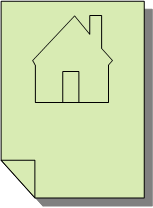
\includegraphics[width=0.25\textwidth]{figures/Homepage-icon.png}
  \end{center}
  \caption{Homepage icon}
  \label{fig:homepageicon}
\end{figure}

\begin{table}[!ht]
  \begin{center}
    \caption{Configurations tested}
    \label{tab:configstested}
    \resizebox{\columnwidth}{!}{%
    \begin{tabular}{l|c} % <-- Alignments: 1st column left, 2nd middle and 3rd right, with vertical lines in between
      \textbf{Configuration} & \textbf{Description} \\
      \hline
      1 & Simple test with one server\\
      2 & Simple test with one server\\
    \end{tabular}
    }
  \end{center}
\end{table}
\sweExpl{Testade konfigurationer}

\section{Implementation …/Modeling/Simulation/…}
\label{sec:implementationDetails}
\sweExpl{Implementering … / modellering / simulering / …}

Two commonly used simulators are:
\begin{description}[labelwidth =\widthof{\textbf{ns-2 or ns-3 simulator}}, leftmargin = !]
    \item[\textbf{Mininet}] This simulator uses traffic control (\texttt{tc}) to simulate network devices connected by links with specific bandwidth, packet loss rates, qdisc methods, etc.
    
    
    \item[\textbf{ns-2 or ns-3 simulator}] These simulators are very useful for simulating wireless communication links between moving devices. You can specify the mobility patterns of the nodes.
\end{description}

\subsection{Some examples of coding}
\engExpl{This section is simply to show some example of how you can include code in your thesis - this is not a section you would have in your thesis.}
\sweExpl{Det här avsnittet är helt enkelt för att visa ett exempel på hur du kan inkludera kod i ditt examensarbete - det här är inte ett avsnitt du skulle ha i ditt examensarbete.}

Listing~\ref{lst:helloWorldInC} shows an example of a simple program written
in C code.

\begin{lstlisting}[language={C}, caption={Hello world in C code}, label=lst:helloWorldInC]
int main() {
printf("hello, world");
return 0;
}
\end{lstlisting}

\engExpl{This template uses the package \texttt{lstlistings} for many different listings. Alternatively, one could use the \texttt{minited} package together with the \texttt{listings} environment, see, for example, \href{https://www.overleaf.com/learn/latex/Code_Highlighting_with_minted}{Code Highlighting with minted}. }

In contrast, Listing~\ref{lst:programmes} is an example of code in Python to
get a list of all of the programs at KTH. Note that on {\DTMsetdatestyle{iso}\DTMdisplaydate{2025}{6}{1}{-1}} the KOPPS API will no longer work.
\engExpl{Note that the change to the iso date format was done in a group so that afterwards the date style returns to what it was, resulting in \DTMdisplaydate{2025}{6}{1}{-1}.}

\lstset{extendedchars=true}  %% This allows character codes in the range 128-255
\begin{lstlisting}[language={Python}, caption={Using a python program to
    access the KTH API to get all of the programs at KTH}, label=lst:programmes]
KOPPSbaseUrl = 'https://www.kth.se'

def v1_get_programmes():
    global Verbose_Flag
    #
    # Use the KOPPS API to get the data
    # note that this returns XML
    url = "{0}/api/kopps/v1/programme".format(KOPPSbaseUrl)
    if Verbose_Flag:
        print("url: " + url)
    #
    r = requests.get(url)
    if Verbose_Flag:
        print("result of getting v1 programme: {}".format(r.text))
    #
    if r.status_code == requests.codes.ok:
        return r.text           # simply return the XML
    #
    return None
\end{lstlisting}
\FloatBarrier

In \Cref{lst:exampleUsingMinted}, line \ref{listinline:ExcelWriter} shows the use of the \texttt{ExcelWriter} function. Line \ref{listinline:UsingToexcel} writes a panda dataframe (named \texttt{comp}) to the spreadsheet, while line \ref{listinline:closingWriter} closes the open spreadsheet.

\begin{listing}[!ht]
\begin{minted}[linenos,breaklines, escapeinside=||]{python}
import pandas as pd
def make_spreadsheet_of_differences(pds):
    global school
    publishers=set()
    writer = pd.ExcelWriter(f'/tmp/{school}_compare_duplicates.xlsx', engine='xlsxwriter') |\label{listinline:ExcelWriter}|
    print("starting")
    for idx, p in enumerate(pds):
        p0=list(p)[0]
        p1=list(p)[1]
        print(f"\nfor {p0} and {p1}")
        comp, publisher1, publisher2=compare_two_records_silent(p0, p1)
        sheet_name=f'{p0}'.split(':')[1]
        print(f'Wrote {sheet_name=}')|\label{listinline:UsingToexcel}|
        comp.to_excel(writer, sheet_name=sheet_name)
        publishers.add(publisher1)
        publishers.add(publisher2)
    
    # Close the Pandas Excel writer and output the Excel file.
    writer.close()|\label{listinline:closingWriter}|
    print(f"{publishers=}")
    return publishers
\end{minted}
\caption{Example of using \texttt{minted} with python code}
\label{lst:exampleUsingMinted}
\end{listing}

\FloatBarrier


\subsection{Some examples of figures in tikz}
\engExpl{This section is simply to show some example of how you can draw your own figures for in your thesis - this is not a section you would have in your thesis.}
\sweExpl{Det här avsnittet är helt enkelt för att visa ett exempel på hur du kan rita dina egna figurer i ditt examensarbete – det här är inte ett avsnitt du skulle ha i ditt examensarbete.}

\Needspace*{5\baselineskip}
These figures are just some examples to show that you can draw your own figures for your thesis. This has two advantages: \first you do not have to worry about copyrights -- as these are your own figures and \Second the text is now readable and not simply a picture of text -- so screen readers can read the figure's contents to someone who is listening to the contents of your thesis.

\subsubsection{Azure's Form Recognizer}
\Cref{fig:processAnInvoice} shows the processing of key-value extraction from a PDF document using Azure's Form Recognizer. 

\tikzset{
    processBox/.style={rectangle, rounded corners, minimum width=3cm, minimum height=1cm,text centered, font=\sffamily, draw=black, fill=red!20},
    largeBox/.style={rectangle, rounded corners, minimum width=3cm, minimum height=4cm,text centered, draw=black}
}
\begin{figure}[!ht]
\resizebox{1.1\textwidth}{!}{%
\begin{tikzpicture}
[align=left,node distance=2cm]

\node (document) [tape,tape bend top=none,draw,font=\sffamily] {PDF\\Document};
\node (GDM) [processBox,  right=0.5cm of document] {OCR};
\node (OCRoutput) [largeBox, right=1cm of GDM] {OCR output};

\node (kvp) [tape,tape bend top=none,draw,font=\sffamily, below=0.25cm of OCRoutput.north] {key-value\\pairs};
\node (entities) [tape,tape bend top=none,draw,font=\sffamily, above=0.35cm of OCRoutput.south] {Entities};
\node (Manual) [processBox, right=1cm of kvp] {Analyze the extracted\\key-value pairs};
\draw [-latex](document) --  (GDM);
\draw [-latex](kvp) --  (Manual);
\path[ draw
     , -latex'] let \p1=(GDM.east), \p2=(kvp.west) in (GDM.east) -- +(0.25*\x2-0.25*\x1, \y1) -- +(0.5*\x2-0.5*\x1, \y2) -- (kvp.west);
\path[ draw
     , -latex'] let \p1=(GDM.east), \p2=(kvp.west), \p3=(entities.west) in (GDM.east) --  +(0.25*\x2-0.25*\x1, \y1) -- +(0.5*\x3-0.5*\x1, \y3) -- (entities.west);
\end{tikzpicture}
}
\caption{The processing of key-value extraction from a PDF document using Azure's Form Recognizer}
  \label{fig:processAnInvoice}
\end{figure}
\FloatBarrier
\subsubsection{Hyper-V with Containers}
 \Cref{fig:hyperVcontainers} shows how Hyper-V deals with containers.
 
 \tikzset{
    container/.style={rectangle, rounded corners, minimum width=2cm, minimum height=1cm,text centered, draw=black, fill=blue!20},
    containerization/.style={rectangle, rounded corners, minimum width=13.25cm, minimum height=1cm,text centered, draw=black, fill=blue!20},
    hypervisor/.style={rectangle, rounded corners, minimum width=13.25cm, minimum height=1cm,text centered, draw=black, fill=red!20},
    os/.style={rectangle, rounded corners, minimum width=13.25cm, minimum height=1cm,text centered, draw=black, fill=orange!20},
    guestos/.style={rectangle, rounded corners, minimum width=2cm, minimum height=1cm,text centered, draw=black, fill=orange!40},
    infrastructure/.style={rectangle, rounded corners, minimum width=13.25cm, minimum height=1cm,text centered, draw=black, fill=green!20},
    hos/.style={rectangle, rounded corners, minimum width=6cm, minimum height=1cm,text centered, draw=black, fill=orange!20},
    kernel/.style={rectangle, rounded corners, minimum width=6cm, minimum height=1cm,text centered, draw=black, fill=purple!20},
    services/.style={rectangle, rounded corners, minimum width=3cm, minimum height=1cm,text centered, draw=black, fill=pink!20]}
}

\begin{figure}[ht!]
    \centering
\resizebox{1\textwidth}{!}{%
\begin{tikzpicture}
[align=center,node distance=2cm]

\node (Infrastructure) [infrastructure, text width=13cm, text centered] {Infrastructure};
\node (OS1) [hos, anchor=north west, align=left, above=1.5cm of Infrastructure.north west, anchor=north west, text width=6cm, text centered] {Host OS};

\node (OS2) [hos, anchor= west, align=left, right=0.5cm of OS1.east, text width=6cm, anchor= west, text centered] {Host OS};

\node (Kernel1) [kernel, anchor=north west, align=left, above=1.5cm of OS1.north east, anchor=north east, text width=3cm, text centered] {Kernel};

\node (Kernel2) [kernel, anchor=north west, align=left, above=1.5cm of OS2.north east, anchor=north east, text width=3cm, text centered] {Kernel};

\node (ServiceA) [container, anchor=east, above=1 cm of Kernel1.east, anchor=east] {Services};
\node (AppA) [container,  left=0.25cm of ServiceA] {App 1};

\node (ServiceB) [container, anchor=east, above=1 cm of Kernel2.east, anchor=east] {Services};
\node (AppB) [container,  left=0.25cm of ServiceB] {App 2};
%\node (AppC) [container,  right=0.25cm of AppB] {App 3};

\draw[black,thick,dashed] ($(OS2.north west)+(-0.3,3.75)$)  rectangle ($(OS2.south east)+(0.5,-0.3)$);
\node[text width=5cm, text=red, above=0.1cm of ServiceB] 
    {\textbf{Container}};

\draw[red,thick,dotted] ($(Kernel2.north west)+(-0.3,1.6)$)  rectangle ($(Kernel2.south east)+(0.3,-0.3)$);
\node[text width=5cm, text=black, above=0.8cm of ServiceB] 
    {\textbf{VM}};
\end{tikzpicture}
}
    \caption{Hyper-V with containers}
    \label{fig:hyperVcontainers}
\end{figure}
\FloatBarrier
\subsubsection{\glsfmtshort{VM} versus Containers}
\Cref{fg:vmsVersusContainers} shows a comparison of virtual machines (VMs) versus containers.

\begin{figure*}[ht!]
    \centering
    \begin{subfigure}[t]{0.5\textwidth}
        \centering
\resizebox{1\textwidth}{!}{%
\begin{tikzpicture}
[align=left,node distance=2cm]

\node (AppA) [container,align=left] {App 1};
\node (AppB) [container,  right=0.25cm of AppA] {App 2};
\node (AppC) [container,  right=0.25cm of AppB] {App 3};

\node (GosA) [guestos,align=left,  below=0.25cm of AppA.south west,anchor=north west] {Guest OS};
\node (GosB) [guestos,  right=0.25cm of GosA] {Guest OS};
\node (GosC) [guestos,  right=0.25cm of GosB] {Guest OS};

\draw [decoration={brace,amplitude=0.5em},decorate, ultra thick,gray, transform canvas={xshift = 0.5cm}]
       (AppC.north -| AppC.east) -- (GosC.south -| AppC.east);
\node[text width=5cm,  right=1cm of GosC.north east] 
    {\textbf{VMs}};

\node (Hypervisor) [hypervisor, anchor=north west, align=left, below=0.25cm of GosA.south west, anchor=north west, text width=13cm, text centered] {Hypervisor};

\node (OS) [os, anchor=north west, align=left, below=0.25cm of Hypervisor.south west, anchor=north west, text width=13cm, text centered] {Host OS};

\node (Infrastructure) [infrastructure, anchor=north west, align=left, below=0.25cm of OS.south west, anchor=north west, text width=13cm, text centered] {Infrastructure};


\end{tikzpicture}
}
        \caption{VM}
    \end{subfigure}%
    ~ 
    \begin{subfigure}[t]{0.5\textwidth}
        \centering
        \resizebox{1\textwidth}{!}{%
\begin{tikzpicture}
[align=left,node distance=2cm]

\node (AppA) [container,align=left] {App 1};
\node (AppB) [container,  right=0.25cm of AppA] {App 2};
\node (AppC) [container,  right=0.25cm of AppB] {App 3};
\node[text width=5cm,  right=0.25cm of AppC] 
    {\textbf{Apps running in Containers}};


\node (Containerization) [containerization, anchor=north west, align=left, below=0.25cm of AppA.south west, anchor=north west, text width=13cm, text centered] {Docker Engine};

\node (OS) [os, anchor=north west, align=left, below=0.25cm of Containerization.south west, anchor=north west, text width=13cm, text centered] {Host OS};

\node (Infrastructure) [infrastructure, anchor=north west, align=left, below=0.25cm of OS.south west, anchor=north west, text width=13cm, text centered] {Infrastructure};


\end{tikzpicture}
}
        \caption{Containers}
    \end{subfigure}
    \caption{Virtual machines (VMs) versus Containers}
    \label{fg:vmsVersusContainers}
\end{figure*}

\cleardoublepage
\chapter{Results and Analysis}
\label{ch:resultsAndAnalysis}
\sweExpl{svensk: Resultat och Analys}

\engExpl{Sometimes this is split into two chapters.\\Keep in mind: How you are going to evaluate what you have done? What are your metrics?\\Analysis of your data and proposed solution\\Does this meet the goals which you had when you started?}

In this chapter, we present the results and discuss them.

\sweExpl{I detta kapitel presenterar vi resultaten och diskutera dem.\\Ibland delas detta upp i två kapitel.\\Hur du ska utvärdera vad du har gjort? Vad är din statistik?\\Analys av data och föreslagen lösning\\Innebär detta att uppfyllelse av de mål som du hade när du började?}

\section{Major results}
\sweExpl{Huvudsakliga resultat}

Some statistics of the delay measurements are shown in Table~\ref{tab:delayMeasurements}.
The delay has been computed from the time the GET request is received until the response is sent.

\sweExpl{Lite statistik av fördröjningsmätningarna visas i Tabell~\ref{tab:delayMeasurements}. Förseningen har beräknats från den tidpunkt då begäran GET tas emot fram till svaret skickas.}

\begin{table}[!ht]
  \begin{center}
    \caption{Delay measurement statistics}
    \label{tab:delayMeasurements}
    \begin{tabular}{l|S[table-format=4.2]|S[table-format=3.2]} % <-- Alignments: 1st column left, 2nd middle and 3rd right, with vertical lines in between
      \textbf{Configuration} & \textbf{Average delay (ns)} & \textbf{Median delay (ns)}\\
      \hline
      1 & 467.35 & 450.10\\
      2 & 1687.5 & 901.23\\
    \end{tabular}
  \end{center}
\end{table}

Table \ref{tab:ping_results} shows the measurement of round trip times from four hosts to and from a server.
\begin{table}[ht!]
\caption[RTT for 4 hosts]{Result for the ping measurements of RTT for 4 hosts} 
\label{tab:ping_results}
\vspace{1em}
\centering
\begin{tabular}{l *{4}{S[table-format=2.3]}}
{} & \multicolumn{4}{c}{host to server RTT in ms} \\
\cmidrule{2-5}
Host & \multicolumn{1}{c}{min}  & \multicolumn{1}{c}{avg} & \multicolumn{1}{c}{max} & \multicolumn{1}{c}{mdev} \\
\midrule
h1 & 5.625 & 5.625 & 5.625 & 0.0 \\
h2 & 2.909 & 2.909 & 1.909 & 0.0 \\
h3 & 5.007 & 5.007 & 5.007 & 0.0 \\
h4 & 2.308 & 2.308 & 2.308 & 0.0 \\
\midrule
\end{tabular}
\end{table}
\FloatBarrier

\sweExpl{Fördröj mätstatistik}
\sweExpl{Konfiguration | Genomsnittlig fördröjning (ns) | Median fördröjning (ns)}

Figure \ref{fig:processing_vs_payload_length} shows an example of the performance as measured in the experiments.

\begin{figure}[!ht]
% GNUPLOT: LaTeX picture
\setlength{\unitlength}{0.240900pt}
\ifx\plotpoint\undefined\newsavebox{\plotpoint}\fi
\begin{picture}(1500,900)(0,0)
\sbox{\plotpoint}{\rule[-0.200pt]{0.400pt}{0.400pt}}%
\put(171.0,131.0){\rule[-0.200pt]{4.818pt}{0.400pt}}
\put(151,131){\makebox(0,0)[r]{ 1.5}}
\put(1419.0,131.0){\rule[-0.200pt]{4.818pt}{0.400pt}}
\put(171.0,212.0){\rule[-0.200pt]{4.818pt}{0.400pt}}
\put(151,212){\makebox(0,0)[r]{ 2}}
\put(1419.0,212.0){\rule[-0.200pt]{4.818pt}{0.400pt}}
\put(171.0,292.0){\rule[-0.200pt]{4.818pt}{0.400pt}}
\put(151,292){\makebox(0,0)[r]{ 2.5}}
\put(1419.0,292.0){\rule[-0.200pt]{4.818pt}{0.400pt}}
\put(171.0,373.0){\rule[-0.200pt]{4.818pt}{0.400pt}}
\put(151,373){\makebox(0,0)[r]{ 3}}
\put(1419.0,373.0){\rule[-0.200pt]{4.818pt}{0.400pt}}
\put(171.0,454.0){\rule[-0.200pt]{4.818pt}{0.400pt}}
\put(151,454){\makebox(0,0)[r]{ 3.5}}
\put(1419.0,454.0){\rule[-0.200pt]{4.818pt}{0.400pt}}
\put(171.0,534.0){\rule[-0.200pt]{4.818pt}{0.400pt}}
\put(151,534){\makebox(0,0)[r]{ 4}}
\put(1419.0,534.0){\rule[-0.200pt]{4.818pt}{0.400pt}}
\put(171.0,615.0){\rule[-0.200pt]{4.818pt}{0.400pt}}
\put(151,615){\makebox(0,0)[r]{ 4.5}}
\put(1419.0,615.0){\rule[-0.200pt]{4.818pt}{0.400pt}}
\put(171.0,695.0){\rule[-0.200pt]{4.818pt}{0.400pt}}
\put(151,695){\makebox(0,0)[r]{ 5}}
\put(1419.0,695.0){\rule[-0.200pt]{4.818pt}{0.400pt}}
\put(171.0,776.0){\rule[-0.200pt]{4.818pt}{0.400pt}}
\put(151,776){\makebox(0,0)[r]{ 5.5}}
\put(1419.0,776.0){\rule[-0.200pt]{4.818pt}{0.400pt}}
\put(171.0,131.0){\rule[-0.200pt]{0.400pt}{4.818pt}}
\put(171,90){\makebox(0,0){ 0}}
\put(171.0,756.0){\rule[-0.200pt]{0.400pt}{4.818pt}}
\put(298.0,131.0){\rule[-0.200pt]{0.400pt}{4.818pt}}
\put(298,90){\makebox(0,0){ 10}}
\put(298.0,756.0){\rule[-0.200pt]{0.400pt}{4.818pt}}
\put(425.0,131.0){\rule[-0.200pt]{0.400pt}{4.818pt}}
\put(425,90){\makebox(0,0){ 20}}
\put(425.0,756.0){\rule[-0.200pt]{0.400pt}{4.818pt}}
\put(551.0,131.0){\rule[-0.200pt]{0.400pt}{4.818pt}}
\put(551,90){\makebox(0,0){ 30}}
\put(551.0,756.0){\rule[-0.200pt]{0.400pt}{4.818pt}}
\put(678.0,131.0){\rule[-0.200pt]{0.400pt}{4.818pt}}
\put(678,90){\makebox(0,0){ 40}}
\put(678.0,756.0){\rule[-0.200pt]{0.400pt}{4.818pt}}
\put(805.0,131.0){\rule[-0.200pt]{0.400pt}{4.818pt}}
\put(805,90){\makebox(0,0){ 50}}
\put(805.0,756.0){\rule[-0.200pt]{0.400pt}{4.818pt}}
\put(932.0,131.0){\rule[-0.200pt]{0.400pt}{4.818pt}}
\put(932,90){\makebox(0,0){ 60}}
\put(932.0,756.0){\rule[-0.200pt]{0.400pt}{4.818pt}}
\put(1059.0,131.0){\rule[-0.200pt]{0.400pt}{4.818pt}}
\put(1059,90){\makebox(0,0){ 70}}
\put(1059.0,756.0){\rule[-0.200pt]{0.400pt}{4.818pt}}
\put(1185.0,131.0){\rule[-0.200pt]{0.400pt}{4.818pt}}
\put(1185,90){\makebox(0,0){ 80}}
\put(1185.0,756.0){\rule[-0.200pt]{0.400pt}{4.818pt}}
\put(1312.0,131.0){\rule[-0.200pt]{0.400pt}{4.818pt}}
\put(1312,90){\makebox(0,0){ 90}}
\put(1312.0,756.0){\rule[-0.200pt]{0.400pt}{4.818pt}}
\put(1439.0,131.0){\rule[-0.200pt]{0.400pt}{4.818pt}}
\put(1439,90){\makebox(0,0){ 100}}
\put(1439.0,756.0){\rule[-0.200pt]{0.400pt}{4.818pt}}
\put(171.0,131.0){\rule[-0.200pt]{0.400pt}{155.380pt}}
\put(171.0,131.0){\rule[-0.200pt]{305.461pt}{0.400pt}}
\put(1439.0,131.0){\rule[-0.200pt]{0.400pt}{155.380pt}}
\put(171.0,776.0){\rule[-0.200pt]{305.461pt}{0.400pt}}
\put(30,453){\rotatebox{-270}{\makebox(0,0){Processing time (ms)}}}
\put(805,29){\makebox(0,0){Payload size (bytes)}}
\put(868.0,131.0){\rule[-0.200pt]{0.400pt}{84.074pt}}
\put(995.0,131.0){\rule[-0.200pt]{0.400pt}{98.287pt}}
\put(1173.0,131.0){\rule[-0.200pt]{0.400pt}{118.041pt}}
\put(1325.0,131.0){\rule[-0.200pt]{0.400pt}{134.904pt}}
\put(1350.0,131.0){\rule[-0.200pt]{0.400pt}{137.795pt}}
\put(1439.0,131.0){\rule[-0.200pt]{0.400pt}{155.380pt}}
\end{picture}
\caption[A GNUplot figure]{Processing time vs. payload length}\vspace{0.5cm}
\label{fig:processing_vs_payload_length}
\end{figure}
\FloatBarrier		

Given these measurements, we can calculate our processing bit rate as the inverse of the time it takes to process an additional byte divided by 8 bits per byte:

\[
	\text{bit rate} = \frac{1}{\frac{\text{time}_{\text{byte}}}{8}} = 20.03 \quad kb/s
\] 

\Cref{tab:majorMarkupLMDetailedResult} shows another table in which some values have been set in bold (using \textbackslash B) to emphasize them. Note how the \texttt{S} formatting has been modified so that it considers the weight of the characters and this is able to decimal align even these hold-faced numbers with the numbers in the column above them.

\begin{table}[!ht]
    \centering
    \caption{Median values of sandwich attributes}
    \label{tab:majorMarkupLMDetailedResult}
    \begin{tabular}{l *{2}{S[detect-weight,mode=text,table-format=3.2]}}
        & \multicolumn{2}{c}{\textbf{sites}}\\
        \cmidrule{2-3}
        \textbf{Attribute} & \textbf{A} & \textbf{B} \\
        \midrule
        price (in SEK) & 36.5 & 71.3 \\
        protean (g) & 97.2 & 100.0 \\
        salt (mg) & 9.7 & 9.3 \\
        \hline
        \textbf{Average customer rating in \%} & \B 82.2 & \B 89.9 \\
        \midrule
    \end{tabular}
\end{table}
\FloatBarrier


\Needspace*{4\baselineskip}
\Cref{fig:stackedrust} shows a stacked bar chart using pgfplots. It illustrates how easy it is to take a set of data and make a stacked bar plot. One of the features is the shifted values -- this is very useful when the bar itself is too small to put the value into.

\pgfplotstableread{
Label Numbers  Refs  Struct/Enum  Heap  Arrays
cratesio 70.04 19.83 8.31 1.3 0.52
librs 49.26 30.49 10.80 7.92 1.53
rustc 55.01 24.80 11.54 6.16 2.49
}\testdata


\pgfkeys{
    /pgf/number format/.cd,
    fixed,
    fixed zerofill,
    precision=2
}
\begin{figure}[ht!]
    \centering
    \scalebox{0.9}{
    \begin{tikzpicture}
    \begin{axis}[
        ybar stacked,
        %reverse legend,
        reverse legend=false,
        %https://tex.stackexchange.com/questions/88892/pgfplots-bar-plot-spacing-inbetween-bars
        enlarge x limits=0.4,
	    bar width=45pt,
        /pgfplots/nodes near coords*/.append style={
        every node near coord/.style={
            color=black,
            font=\small,
            name=X,
%            shift={    
%                (50pt,25pt)
%                },
            xshift={50pt},
                yshift ={
                ifthenelse((\plotnum == 4), 30pt,20pt)},
            },
            scatter/@post marker code/.append code={
                \node(Y){};
                \draw(X)--(Y.center);
            }
        },
	    nodes near coords,
        bar shift=5pt,
        ymin=0,
        ymax=115,
        xtick=data,
        width=1\textwidth,
        legend style={draw=none},
        legend image post style={scale=2.0},
        legend style={
            at={(0.5,-0.2)},
            anchor=north,
            legend columns=-2,
            font=\large,
            %mark size=20pt,
        },
        ylabel=Percentage points (\%),
        xticklabels from table={\testdata}{Label},
        xticklabel style={rotate=30},
    ]
    \addplot  table [y=Numbers, meta=Label, x expr=\coordindex] {\testdata};
    \addlegendentry{Numbers}
    \addplot table [y=Refs, meta=Label, x expr=\coordindex] {\testdata};
    \addlegendentry{Refs}
    \addplot  table [y=Struct/Enum, meta=Label, x expr=\coordindex] {\testdata};
    \addlegendentry{Struct/Enum}
    \addplot  table [y=Heap, meta=Label, x expr=\coordindex] {\testdata};
    \addlegendentry{Heap}
    \addplot  table [y=Arrays, meta=Label, x expr=\coordindex] {\testdata};
    \addlegendentry{Arrays}
    \end{axis}
    \end{tikzpicture}}
\caption{Rust types distribution for the compiler, crates.io, and lib.rs.
(percentage) - appears here with the permission of the author - see the thesis at \url{https://urn.kb.se/resolve?urn=urn\%3Anbn\%3Ase\%3Akth\%3Adiva-332124}}
\label{fig:stackedrust}
\end{figure}
\FloatBarrier



\section{Reliability Analysis}
\sweExpl{Analys av tillförlitlighet\\
Tillförlitlighet i metod och data}

\section{Validity Analysis}
\sweExpl{Analys av validitet\\
Validitet i metod och data}

\cleardoublepage
\chapter{Discussion}
\label{ch:discussion}
\sweExpl{Diskussion\\
Förbättringsförslag?}
\generalExpl{This can be a separate chapter or a section in the previous chapter.}

\cleardoublepage
\chapter{Conclusions and Future work}
\label{ch:conclusionsAndFutureWork}
\sweExpl{Slutsats och framtida arbete}

\generalExpl{Add text to introduce the subsections of this chapter.}

\section{Conclusions}
\label{sec:conclusions}
\sweExpl{Slutsatser}
\engExpl{Describe the conclusions (reflect on the whole introduction given in Chapter 1).}


  
\engExpl{Discuss the positive effects and the drawbacks.\\
Describe the evaluation of the results of the degree project.\\
Did you meet your goals?\\
What insights have you gained?\\
What suggestions can you give to others working in this area?\\
If you had it to do again, what would you have done differently?}

\sweExpl{Uppfyllde du dina mål?\\
Vilka insikter har du fått?\\
Vilka förslag kan du ge till andra som arbetar inom detta område?
Om du skulle göra detta igen, vad skulle du ha gjort annorlunda?}

\section{Limitations}
\label{sec:limitations}
\sweExpl{Begränsande faktorer\\Vad gjorde du som begränsade dina ansträngningar? Vilka är begränsningarna i dina resultat?}
\engExpl{What did you find that limited your efforts? What are the limitations of your results?}


\section{Future work}
\label{sec:futureWork}
\sweExpl{Vad du har kvar ogjort?\\Vad är nästa självklara saker som ska göras?\\Vad tips kan du ge till nästa person som kommer att följa upp på ditt arbete?}
\engExpl{Describe valid future work that you or someone else could or should do.\\
Consider: What you have left undone? What are the next obvious things to be done? What hints can you give to the next person who is going to follow up on your work?}



Due to the breadth of the problem, only some of the initial goals have been
met. In these section we will focus on some of the remaining issues that
should be addressed in future work. ...

\subsection{What has been left undone?}
\label{what-has-been-left-undone}

The prototype does not address the third requirment, \ie a yearly unavailability of less than 3 minutes; this remains an open problem. ...

\subsubsection{Cost analysis}
\generalExpl{Example of a missing component}
The current prototype works, but the performance from a cost perspective makes this an impractical solution. Future work must reduce the cost of this solution; to do so, a cost analysis needs to first be done. ...

\subsubsection{Security}
\generalExpl{Example of a missing component}
A future research effort is needed to address the security holes that results from using a self-signed certificate. Page filling text mass. Page filling text mass. ...


\subsection{Next obvious things to be done}

In particular, the author of this thesis wishes to point out xxxxxx remains as a problem to be solved. Solving this problem is the next thing that should be done. ...

\section{Reflections}
\label{sec:reflections}
\sweExpl{Reflektioner}
\sweExpl{Vilka är de relevanta ekonomiska, sociala, miljömässiga och etiska aspekter av ditt arbete?}
\engExpl{What are the relevant economic, social,
  environmental, and ethical aspects of your work?
}



One of the most important results is the reduction in the amount of
energy required to process each packet while at the same time reducing the
time required to process each packet.

The thesis contributes to the \gls{UN}\enspace\glspl{SDG} numbers 1 and 9 by
xxxx. 




\noindent\rule{\textwidth}{0.4mm}
\engExpl{In the references, let Zotero or other tool fill this in for you. I suggest an extended version of the IEEE style, to include URLs, DOIs, ISBNs, etc., to make it easier for your reader to find them. This will make life easier for your opponents and examiner. \\IEEE Editorial Style Manual: \url{https://www.ieee.org/content/dam/ieee-org/ieee/web/org/conferences/style_references_manual.pdf}}
\sweExpl{Låt Zotero eller annat verktyg fylla i det här för dig. Jag föreslår en utökad version av IEEE stil - att inkludera webbadresser, DOI, ISBN osv. - för att göra det lättare för läsaren att hitta dem. Detta kommer att göra livet lättare för dina opponenter och examinator.}

\cleardoublepage
% Print the bibliography (and make it appear in the table of contents)
\renewcommand{\bibname}{References}


\iftoggle{biblatex}{
    %\typeout{Biblatex current language is \currentlang}
    \printbibliography[heading=bibintoc]
}{
    \phantomsection  % make it include a hyperref - see https://tex.stackexchange.com/a/98995
    \addcontentsline{toc}{chapter}{References}
    \bibliography{references}
}



\warningExpl{If you do not have an appendix, do not include the \textbackslash cleardoublepage command below; otherwise, the last page number in the metadata will be one too large.}
\cleardoublepage
\appendix
\renewcommand{\chaptermark}[1]{\markboth{Appendix \thechapter\relax:\thinspace\relax#1}{}}
\chapter{Supporting materials}
\label{sec:supportingMaterial}
\generalExpl{Here is a place to add supporting material that can help others build upon your work. You can include files as attachments to the PDF file or indirectly via URLs. Alternatively, consider adding supporting material uploaded as separate files in DiVA.}

% Attach the BibTeX for your references to make it easy for a reader to find and use them
The BibTeX references used in this thesis are attached. \attachfile[description={references.bib}]{references.bib}

% Attach source code file(s) or add a URL to the github or other repository
Some source code relevant to this project can be found at \url{https://github.com/gqmaguirejr/E-learning} and \url{https://github.com/gqmaguirejr/Canvas-tools}.

Your reader can access the attached (embedded) files using a PDF tool such as Adobe Acrobat Reader using the paperclip icon in the left menu, as shown in \Cref{fig:PDFreaderPaperclipExample} or by right-clicking on the push-pin icon in the PDF file and then using the menu to save the embedded file as shown in \Cref{fig:PDFreaderPushpinExample}.

An argument for including supporting material in the PDF file is that it will be available to anyone who has a copy of the PDF file. As a result, they do not have to look elsewhere for this material. This comes at the cost of a larger PDF file. However, the embedded files are encoded into a compressed stream within the PDF file; thus, reducing the number of additional bytes. For example, the references.bib file that was used in this example is \SI{10617}{\byte} in size but only occupies \SI{4261}{\byte} in the PDF file.

\warningExpl{DiVA is limited to $\approx$\SI{1}{\giga\byte} for each supporting file. If you have very large amounts of supporting material, you will probably want to use one of the data repositories. For additional help with this, contact KTH Library via 
\href{mailto:researchdata@kth.se}{researchdata@kth.se}.\\As of Spring 2024, there are plans to migrate this supporting data from DiVA to a research data repository.
}

\begin{figure}[!ht]
  \begin{center}
    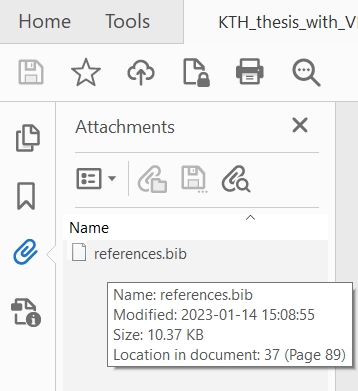
\includegraphics[width=0.50\textwidth]{README_notes/pdf-viewer-attached-files.png}
  \end{center}
  \caption{Adobe Acrobat Reader using the paperclip icon for the attached references.bib file}
  \label{fig:PDFreaderPaperclipExample}
\end{figure}
\FloatBarrier

\begin{figure}[!ht]
  \begin{center}
    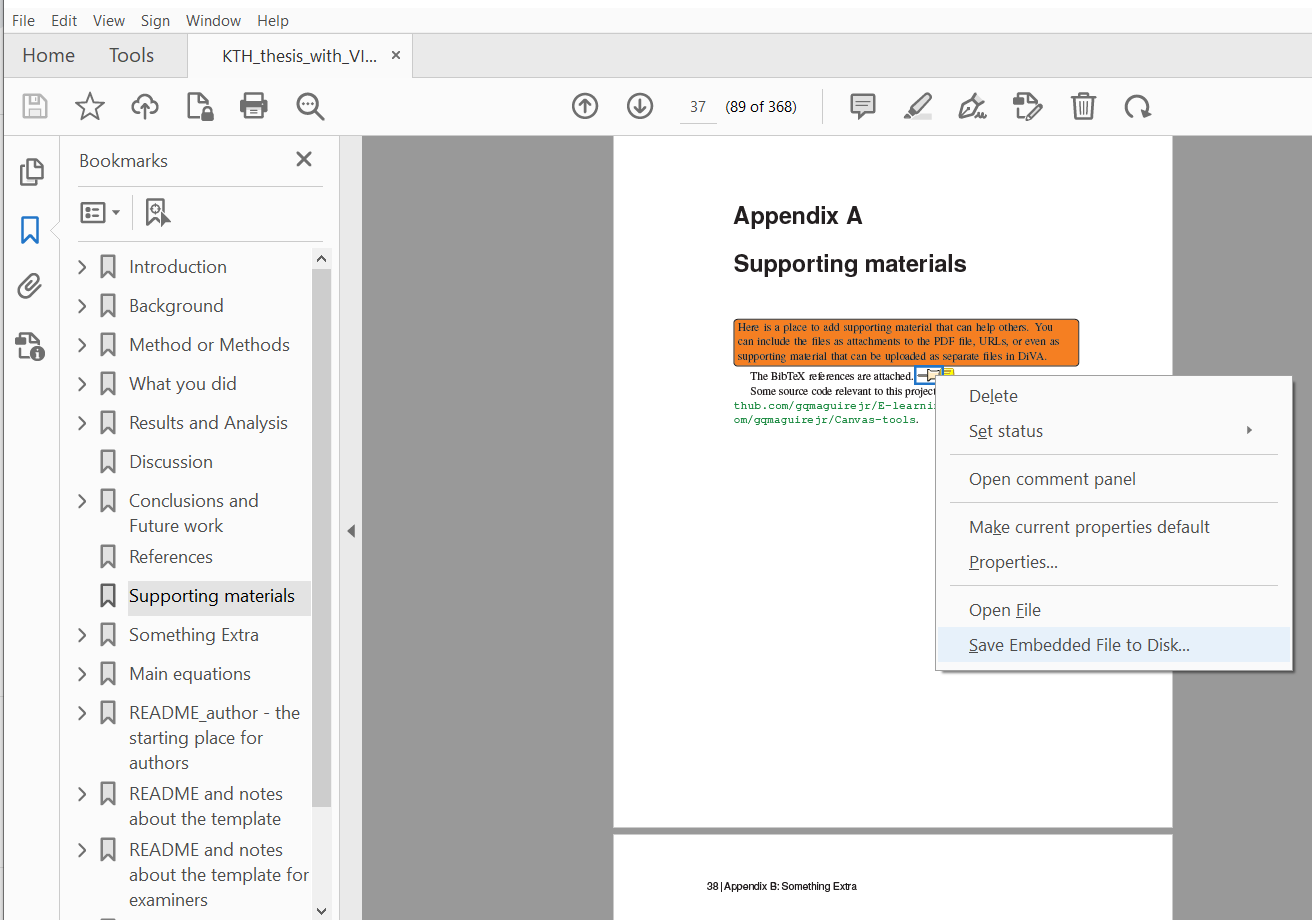
\includegraphics[width=0.99\textwidth]{README_notes/Bib-save-embedded-example.png}
  \end{center}
  \caption{Adobe Acrobat Reader after right-clicking on the push-pin icon for the attached references.bib file}
  \label{fig:PDFreaderPushpinExample}
\end{figure}
\FloatBarrier
\cleardoublepage

\chapter{Something Extra}
\sweExpl{svensk: Extra Material som Bilaga}

\section{Just for testing KTH colors}
\iftoggle{digitaloutput}{
    \textbf{You have selected to optimize for digital output}
}{
    \textbf{You have selected to optimize for print output}
}

\begin{itemize}[noitemsep]
    \item Primary color
    \begin{itemize}
    \item \textcolor{kth-blue}{kth-blue \iftoggle{digitaloutput}{
    actually Deep sea
    }{}} {\color{kth-blue} \rule{0.3\linewidth}{1mm} }\\

    \item \textcolor{kth-blue80}{kth-blue80} {\color{kth-blue80} \rule{0.3\linewidth}{1mm} }\\
\end{itemize}

\item  Secondary colors
\begin{itemize}[noitemsep]
    \item \textcolor{kth-lightblue}{kth-lightblue \iftoggle{digitaloutput}{
    actually Stratosphere
    }{}} {\color{kth-lightblue} \rule{0.3\linewidth}{1mm} }\\

    \item \textcolor{kth-lightred}{kth-lightred \iftoggle{digitaloutput}{
    actually Fluorescence}{}} {\color{kth-lightred} \rule{0.3\linewidth}{1mm} }\\

    \item \textcolor{kth-lightred80}{kth-lightred80} {\color{kth-lightred80} \rule{0.3\linewidth}{1mm} }\\

    \item \textcolor{kth-lightgreen}{kth-lightgreen \iftoggle{digitaloutput}{
    actually Front-lawn}{}} {\color{kth-lightgreen} \rule{0.3\linewidth}{1mm} }\\

    \item \textcolor{kth-coolgray}{kth-coolgray \iftoggle{digitaloutput}{
    actually Office}{}} {\color{kth-coolgray} \rule{0.3\linewidth}{1mm} }\\

    \item \textcolor{kth-coolgray80}{kth-coolgray80} {\color{kth-coolgray80} \rule{0.3\linewidth}{1mm} }
\end{itemize}
\end{itemize}

\textcolor{black}{black} {\color{black} \rule{\linewidth}{1mm} }

% Include an example of using nomenclature
\ifnomenclature
    \cleardoublepage
    \chapter{Main equations}
    \label{ch:NomenclatureExamples}
    This appendix gives some examples of equations that are used throughout this thesis.
    \section{A simple example}
    The following example is adapted from Figure 1 of the documentation for the package nomencl (\url{https://ctan.org/pkg/nomencl}).
    \begin{equation}\label{eq:mainEq}
    a=\frac{N}{A}
    \end{equation}
    \nomenclature{$a$}{The number of angels per unit area\nomrefeq}%       %% include the equation number in the list
    \nomenclature{$N$}{The number of angels per needle point\nomrefpage}%  %% include the page number in the list
    \nomenclature{$A$}{The area of the needle point}%
    The equation $\sigma = m a$%
    \nomenclature{$\sigma$}{The total mass of angels per unit area\nomrefeqpage}%
    \nomenclature{$m$}{The mass of one angel}
follows easily from \Cref{eq:mainEq}.

    \section{An even simpler example}
    The formula for the diameter of a circle is shown in \Cref{eq:secondEq} area of a circle in \cref{eq:thirdEq}.
    \begin{equation}\label{eq:secondEq}
    D_{circle}=2\pi r
    \end{equation}
    \nomenclature{$D_{circle}$}{The diameter of a circle\nomrefeqpage}%
    \nomenclature{$r$}{The radius of a circle\nomrefeqpage}%

    \begin{equation}\label{eq:thirdEq}
    A_{circle}=\pi r^2
    \end{equation}
    \nomenclature{$A_{circle}$}{The area of a circle\nomrefeqpage}%

    Some more text that refers to \eqref{eq:thirdEq}.
\fi  %% end of nomenclature example

\cleardoublepage
% Information for authors
%\include{README_author}
\subfile{README_author}

\cleardoublepage
% information about the template for everyone
\input{README_notes/README_notes}

\begin{comment}
% If you actually want to have the full table of National Subject Categories (temporarily) include this appendix
\subfile{README_notes/National_Subject_Categories}
\cleardoublepage
\end{comment}

\begin{comment}
% Information for examiners
\ifxeorlua
\cleardoublepage
\input{README_notes/README_examiner_notes}
\fi
\end{comment}

\begin{comment}
% Information for administrators
\ifxeorlua
\cleardoublepage
\input{README_notes/README_for_administrators.tex}
\fi
\end{comment}

\begin{comment}
% Information for Course Coordinators
\ifxeorlua
\cleardoublepage
\input{README_notes/README_for_course_coordinators}
\fi
\end{comment}

%% The following label is necessary for computing the last page number of the body of the report to include in the "For DIVA" information
\label{pg:lastPageofMainmatter}

\cleardoublepage
\clearpage\thispagestyle{empty}\mbox{} % empty page with backcover on the other side
\kthbackcover
\fancyhead{}  % Do not use header on this extra page or pages
\section*{€€€€ For DIVA €€€€}
\lstset{numbers=none} %% remove any list line numbering
\divainfo{pg:lastPageofPreface}{pg:lastPageofMainmatter}

% If there is an acronyms.tex file,
% add it to the end of the For DIVA information
% so that it can be used with the abstracts
% Note that the option "nolol" stops it from being listed in the List of Listings

% The following bit of ugliness is because of the problems PDFLaTeX has handling a non-breaking hyphen
% unless it is converted to UTF-8 encoding.
% If you do not use such characters in your acronyms, this could be simplified.
\ifxeorlua
\IfFileExists{lib/acronyms.tex}{
\section*{acronyms.tex}
\lstinputlisting[language={[LaTeX]TeX}, nolol, basicstyle=\ttfamily\color{black},
commentstyle=\color{black}, backgroundcolor=\color{white}]{lib/acronyms.tex}
}
{}
\else
\IfFileExists{lib/acronyms-for-pdflatex.tex}{
\section*{acronyms.tex}
\lstinputlisting[language={[LaTeX]TeX}, nolol, basicstyle=\ttfamily\color{black},
commentstyle=\color{black}, backgroundcolor=\color{white}]{lib/acronyms-for-pdflatex.tex}
}
{}
\fi


\end{document}
